\chapter{Modèle de décision basé sur les comportements de dominance}
	\label{chap:dec}
	\markboth{DÉCISION BASÉE SUR LA DOMINANCE}{DÉCISION BASÉE SUR LA DOMINANCE}
	
	\begingroup
	\parindent=0em
	\etocsettocstyle{\rule{\linewidth}{\tocrulewidth}\vskip0.5\baselineskip}{\rule{\linewidth}{\tocrulewidth}}
	\localtableofcontents 
	\clearpage
	\endgroup
	%Après avoir défini la relation interpersonnelle de dominance dans le chapitre \ref{chap:etat}, ainsi que sa manifestation dans l'interaction tant sur l'aspect verbal que non verbal, nous avons ensuite détaillé son impact sur les stratégies de négociations. 
	
	Ce chapitre présente le modèle de décision d'un agent négociateur qui lui permet d'adapter sa stratégie de négociation à la relation de dominance qu'il vise à instaurer avec son interlocuteur. Dans la section 1, nous définissons les principes de décisions basés sur les comportements de dominance inspirés des travaux en psychologie sociale. Dans la section 2, nous présentons un premier modèle décisionnel utilisant des règles de décisions.  Pour ce modèle, nous nous sommes basés sur la structure d'arbres défini dans \emph{DISCO} \cite{rich09} et nous discuterons ses limites. Ensuite dans la section 3, nous présenterons notre modèle décisionnel final qui prends en compte les comportements de dominance de l'agent associés à ses préférences pour construire sa stratégie de négociation. Enfin, nous présenterons deux études visant à valider le modèle décisionnel dans les deux cas d'interaction agent/agent et agent/humain.
	
	\section{Comportements de dominance et stratégies de négociation}
	\label{chap:domer}
	Comme nous l'avons présenté dans le chapitre 2  %\ref{chap:etat}
	, nous nous sommes essentiellement basés sur les travaux en psychologie sociale pour la définition de la dominance. 
	La dominance comme relation interpersonnelle est présentée comme la capacité à exprimer des comportements verbaux et non verbaux par lesquels l'influence est atteinte \cite{burgoon2006nonverbal}. Prenant cette définition comme point de départ, nous nous sommes ensuite intéressé à la manifestation des comportements de dominance durant le processus de négociation et comment ces comportements influençaient les stratégies de négociations dans le contexte d'interaction humain/humain. 
	
	Dans ce qui suit, nous présentons \emph{trois principes} de comportements extraits des travaux en psychologie sociale qui ont étudiaient l'impact des comportements de dominance sur les négociateurs et leur stratégies.
	
	\begin{enumerate}
		\item \textbf{Niveau d'exigence et de concessions:} Les négociateurs dominants affichent un niveau d'exigence plus important comparés aux négociateurs soumis. Par ailleurs, les exigences des négociateurs soumis diminuent avec le temps. Ceci se traduit par des concessions plus importantes comparés aux négociateurs plus dominants. \cite{de1995impact}
		
		\item \textbf{Soi \emph{vs} autrui:} Les négociateurs soumis prennent en compte les préférences de leur interlocuteur dans la négociation, tandis que les négociateurs  dominants sont centrés sur eux-mêmes et s'intéressent uniquement à la satisfaction leurs propres préférences. \cite{fiske1993controlling,de1995impact}
		
		\item \textbf{Contrôle du flux de la négociation:}
		Les négociateurs dominant ont tendance à faire le premier pas et à prendre les devants dans la négociation \cite {magee2007power}. Ils sont centrés sur l'avancement du processus de prise de décision, en prenant des décisions rapides \cite{zablotskaya2012relating}.
		A l'opposé, les négociateurs moins dominants visent à construire un modèle précis des préférences du partenaire de négociation. 
		Par conséquent,  ils posent plus de questions afin de collecter les informations nécessaires qui leurs permettent de prendre la décision la plus équitable(\emph{e.g}  faire des propositions)~\cite{de2004influence}. 
		
	\end{enumerate}
	
	
	Notre but est de construire un modèle de décision capable d'illustrer ces comportements de dominance et par conséquent, adapter la stratégie de négociation en fonction de la dominance de l'agent.
	
	Dans ce qui suit nous présenterons le modèle décision de l'agent qui prend en compte la relation de dominance.
	
	
	\section{Règles de décision}
	Dans le cadre de cette thèse, nous avons construit un premier modèle de décisions composé de règles de décision modélisées sous forme d'arbres de dialogues. L'implémentation de notre système de dialogue est géré par le logiciel \emph{Disco} \cite{rich09}. Disco est une implémentation d'un ``collaborative discourse manager'' inspiré d'une théorie de dialogue collaboratif comme \emph{Collagen} \cite{rich1997collagen}. Disco est un système qui permet la génération de dialogues orienté tâches pour lequel il utilise le formalisme d'arbre hiérarchique pour la gestion des tâches. Il est implémenté avec le standard ANSI/CEA-2018 : chaque tâche est définit avec des préconditions, des effets et des postconditions. Les tâches sont regroupées par \emph{recettes} munies de conditions d'applicabilité.
	
	De plus, \emph{Disco} a été étendu avec un module génération d'arbres de dialogues afin de communiquer et collaborer avec l'utilisateur pour la réalisation des tâches. Ce module est nommé Disco for Games (D4g) et permet de définir des sémantiques d'actes de dialogue. 
	
	Nous avons complété ce système avec les actes de dialogues présenté dans la section \ref{sec:communication} afin qu'il puisse supporter la négociation sur les préférences.
	
	Pour chaque acte de dialogue que l'agent reçoit, nous modélisons des règles de décisions sous forme d'arbre de décisions pour permettre à l'agent de décider du prochain acte de dialogue à énoncer.
	Chaque branchement dans l'arbre dispose d'une condition d'applicabilité. Cette dernière prend en compte le contexte courant de la négociation. De plus, elle prend en compte la position de l'agent dans le spectre de dominance pour exprimer des stratégies de négociation compatibles avec sa relation de dominance.
	%Par exemple, suite à un acte \emph{Propose} énoncé par l'utilisateur, l'agent peut répondre par un \emph{Accept}, un \emph{Reject} ou un autre \emph{Propose}. 
%	Par exemple:
%	\begin{verbatim}
%	User: "Je propose que nous allions dans un restaurant Chinois." 
%		Agent: "je propose que nous allions plutôt dans un restaurant
%			   Japonais". 
%	\end{verbatim}

	
	
	\subsection{Sélection de l'acte de dialogue}
	Nous avons initialisé l'agent avec un comportement de dominance parmi trois types de comportements inspirés de la littérature en psychologies social.  L'agent peut suivre un comportement \emph{dominant, soumis} ou \emph{neutre}. 
	
	En fonction de l'acte de dialogue que l'agent reçoit, nous générons un ensemble de réponses possibles. Chaque réponse dépend de la position de dominance initiale de l'agent. Le système de dialogue offre à l'utilisateur la liberté de choisir n'importe quel acte de dialogue pour son tour de parole. Disco déroule alors l'arbre de dialogue correspondant de gauche à droite (en commençant par la branche la plus à gauche). La première branche applicable rencontrée est directement exécutée sans vérifier les branches restantes.
	
	Notons que dans la suite, chaque arbre de dialogue est défini avec une condition de sortie qui clos la négociation avec un échec. Cette dernière est activée seulement par agent \emph{dominant} dans la situation où toutes les valeurs restantes ne sont pas acceptables. 
	
	\subsubsection{AskPreference}
		Quand l'agent reçoit un \emph{AskPreference} de la part de son interlocuteur, la réponse de l'agent consistera à donner son avis sur la question: partager ses préférences sur la question demandée. Par exemple: 
		
		\begin{verbatim}
			User : AskPreference(Japanese) 
					"Do you like Japanese cuisine ?"
			Agent : StatePreference(Japanese, true)
					"I like Japanese cuisine."
		\end{verbatim}
	

		 
		 
	\subsubsection{State Preference(v)}
		Durant le processus de négociation, les négociateurs partagent des informations sur leurs préférences via des \emph{StatePreference(v)}. Par conséquent, quand l'agent reçoit ce type d'acte de dialogue, il a le choix entre deux stratégies possibles. Nous utiliserons l'exemple où l'interlocuteur ait exprimé  \emph{StatePreference(calme, true)} (I like calm restaurants) pour illustrer les choix de l'agent. 
		
		
		\paragraph{ i. Actes de négociations :}
			L'agent peut décider d'utiliser des actes de négociations et plus précisément un \emph{Propose} suite à la reception d'un \emph{StatePreference} pour deux raisons relatives à ses comportements de dominance. Nous présentons ci dessous les conditions d'applicabilités ainsi que la valeur associée à l'acte dialogique \emph{Propose}. 
			\begin{itemize}
				
				\item L'agent propose la valeur $v$ exprimée par l'interlocuteur. La condition d'applicabilité repose sur l'acceptabilité de la valeur $v$. En effet, si l'interlocuteur énonce apprécier $v$ et que dans l'état mental de l'agent $v$ est satisfiable, l'agent proposera donc de choisir la valeur $v$. Par exemple, suite au \emph{StatePreference(calme, true)} énoncé par l'interlocuteur, si $Italian$ est acceptable pour l'agent, il énoncera un \emph{Propose(Italian)} au prochain tour. Ce comportement traduit le premier principe qui stipule que l'agent prend en compte les préférences de son interlocuteur dans la prise de décision.
				
				\item Le second cas illustre le troisième principe. En effet, dans un processus de négociation, plus l'agent est dominant, plus il veut prendre le contrôle de la négociation et faire avancer la prise de décision le plus rapidement possible. Ceci se traduit par des expressions de \emph{Propose} jusqu'a arriver à un compromis.
				Pour ce faire, l'agent analyse le contexte de la négociation afin d'évaluer s'il a collecté les informations suffisantes (les tours de \emph{StatePreferences}) pour prendre une décision équitable. Nous avons proposé ce simple algorithme (voir figure \ref{alg:maxtours}),qui définit un nombre maximums de tours de paroles réservé à l'échange d'information. Cet algorithme prend en compte les comportements de dominance de l'agent. En effet, plus l'agent est soumis, plus il va chercher à collecter le maximum d'informations comme le spécifie le principe 3. 
				
				Une fois le nombre de tous maximum alloués à l'échange d'informations atteint, l'agent énonce une proposition avec une valeur acceptable. 
								
			\end{itemize}
			
			
		\paragraph{ii. Partager des préférences:} Cette stratégie est activée si aucune condition d'applicabilité n'est satisfaite dans la première stratégie. 
		L'agent peut échanger des informations sur les préférences dans le but d'optimiser ses décisions pour un solution équitable. En fonction de contexte de la négociation l'agent peut choisir un acte de dialogue précis.
			\begin{enumerate}
				\item \emph{StatePreference(v)}: La première réponse possible est de partager ses préférences la valeur communiqué par l'interlocuteur. Pour cela, une condition d'applicabilité est définie. En effet, il faut que $v \notin S_i$, c'est à dire que l'agent n'ait pas déjà communiqué son avis sur la valeurs $v$ comme présenté dans la figure \ref{fig:SP}. Dans notre exemple, cela voudrait dire que l'agent n'a pas encore partagé son avis sur la cuisine italienne.
				Cependant, si cette condition d'applicabilité n'est pas vérifiée (l'agent a déjà parlé de la cuisine italienne dans la négociation), l'agent peut échanger des informations sur d'autres valeurs en fonction de sa valeur de dominance. 
				
				\item \emph{StatePreference (x)}: l'agent est \emph{neutre}, il va exprimer ses préférences sur des valeurs qu'il n'a pas encore communiqués $x \notin S_i$ afin d'inciter son interlocuteur à partager des informations sur ses préférences.
				\item \emph{AskPreference (x)}: l'agent est \emph{soumis}, il va respecter le principe 3 et essayer de collecter des informations sur les préférences de son interlocuteur $x \not \in (U_i or A_i)$.
			\end{enumerate}  
	
	\begin{figure}[t]
		\caption{\label{alg:maxtours} Maximum de tours de \emph{StatePreference} autorisé en fonction des comportements de dominance de l'agent}
		\begin{algorithmic}[1]
			\Function{MaxStatements}{}
			\State $nbTours$ = Nombre de \emph{StatePreferences} exprimés successivement.
			\State $maxTours$ 
			\If{($dominant$)} 
			\State $maxTours = 1$
			\EndIf
			\If{($peer$)} \State $maxTours = 2$
			\EndIf
			\If{($soumis$)} 
			\State $maxTours = 4$
			\EndIf
			\State $retrun$ $nbTours\geq maxTours$
			\EndFunction
		\end{algorithmic}
	\end{figure} 
	
	
%	\begin{figure}[!t]
%		\centering
%		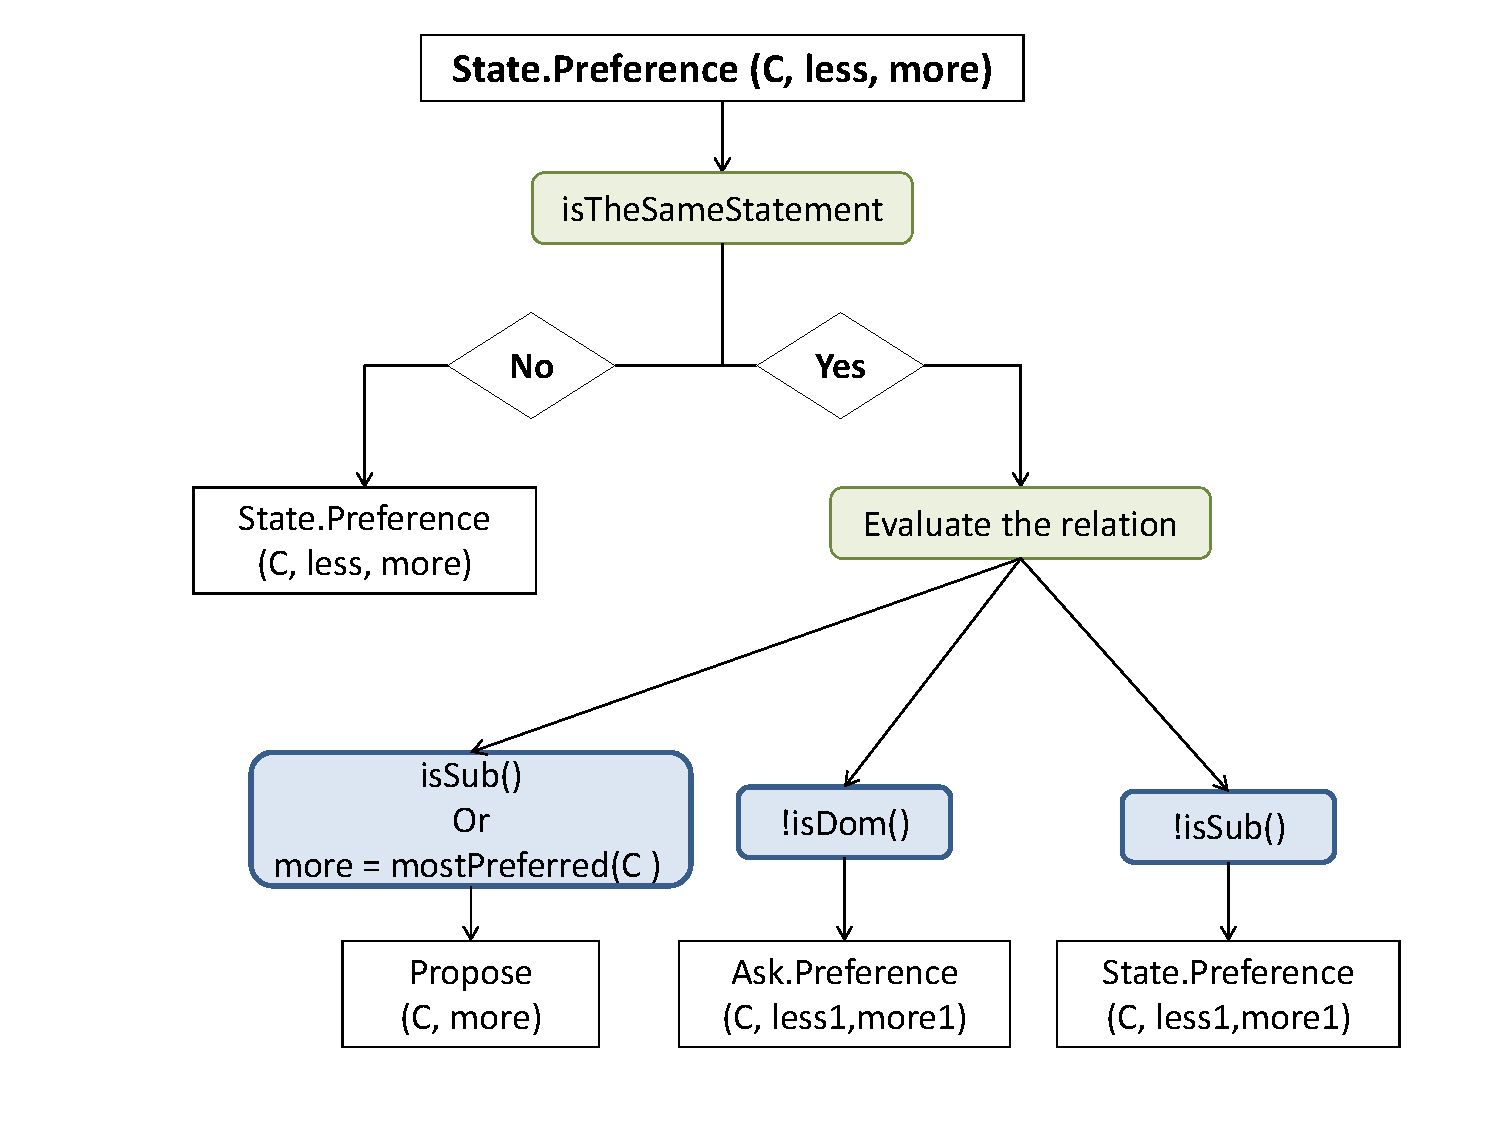
\includegraphics[width=4.5in] {Figures/chap4/statePref.pdf}
%		\caption{Les réponses générés suite à un StatePreference}
%		\label{fig:SP}
%	\end{figure}
%	
	
	
	
	 
	\subsubsection{Propose}
	A la réception d'un \emph{Propose}, l'agent doit décider d'accepter ou refuser la proposition. En conséquence, il choisit une réponse en fonction de ses comportements de dominance.
	
	Pour calculer l'acceptabilité de l'offre reçue, l'agent met en application le principe 2. En fonction de sa dominance, l'agent a niveau d'exigence et de concessions. 
	\paragraph{i. Niveau de concessions}
	
	Au fur et à mesure que la négociation évolue, si un compromis n'est pas trouvé, l'agent sera amené à faire des concessions sur certains critères. L'agent dispose de relations de préférences sur les critères. Par exemple, il peut considérer que le type de cuisine est le critère le plus important pour choisir un restaurant. En fonction de son ordre de préférences et de sa dominance, l'agent peut faire des concessions sur des critères et ne plus les considérer comme importants dans sa prise de décision. C'est à dire, pour un critère donné, il va considérer que toutes les valeurs de ce critères sont maintenant acceptables. 
	Par exemple, il peut considérer que le critère de \emph{localisation} n'est plus important pour le choix d'un restaurant. Par conséquent, il considérera que toute valeur de \emph{localisation} est désormais \emph{acceptable}.
	
	Nous présentons dans la figure \ref{alg:important}, l'algorithme pour calculer si un critère est toujours important compte tenu l'état courant de la négociation. L'agent dominant est conçu pour considérer tout les critères importants. Cependant, un agent neutre ou soumis augmentera ses concessions en fonction de l'évolution de la négociation. 
	
	\begin{figure}[h]
		\caption{\label{alg:important} Calcul de l'importance d'un critère $C$}
		\begin{algorithmic}[1]
			\Function{isImportant}{$C$}
			\State $nbProposal = |P| + |R|$ 
			\Comment{Les propositions non acceptées durant la négociation}
			\State criteria = trier les critères par ordre décroissant de préférences
			\State $minProposals$ \Comment{Le nombre minimums de propositions pour activer la concession}
			\If{($dominant$ \textbf{OR} $nbProposal < minProposals$}) 
			\State $true$ \Comment{L'agent dominant ne fait pas de concessions}
			\Else
			\State $concession $ = ($nbProposal - minProposal$)/ $minProposal$
			\State return $rank(C) < |\mathcal{C}| - concession$
			\EndIf 
			\EndFunction
		\end{algorithmic}
	\end{figure}
	
	\paragraph{ii. Niveau d'exigence}
		Une fois que l'agent décide si un critère est important (dans le cadre d'une proposition concernant une valeur de critère), l'agent calcule l'acceptabilité de cette valeur en fonction de son niveau d'exigence. Plus l'agent est dominant plus il est exigent et donc tend à avoir un ensemble restreints de valeurs acceptables. Nous avons écrit un algorithme simple, présenté dans la figure \ref{alg:pseudo} pour simuler ce comportement d'exigence. 
	
	En fonction du résultat obtenu à partir de ces deux fonctions, l'agent définit sa stratégie de réponse: 
	
	\begin{itemize}	
		\item  \emph{Accept(p)}: Si la proposition \emph{p} est acceptable, l'agent accepte la proposition via l'acte de dialogue un \emph{Accept(p)}. Sinon, l'agent doit faire évoluer la négociation pour trouver un meilleurs compromis. 
		\item \textbf{Stratégie de rejet :} En fonction de sa dominance, l'agent rejette une proposition de différentes manières:
		\begin{itemize}[label= $\circ$]
			\item \emph{AskPreference(v)} l'agent est \emph{soumis}, il choisis alors d'énoncer un acte de dialogue \emph{Ask} tel que $v \not\in (U_i or A_i)$. Les personnes soumises ont tendance à ne pas exprimer leurs opinions ouvertement. Pour cela, au lieu de rejeter une proposition non acceptable, l'agent change le sujet de négociation et active le principe 3 pour collecter plus de connaissances sur les préférences de son interlocuteur. Cette branche est applicable uniquement quand l'agent reçoit une proposition pour la première fois où il a déjà refusé deux propositions.  
			
			\item \emph{Reject(p)}: l'agent est \emph{neutre} ou \emph{soumis}. Par conséquent, sa stratégie consistera à rejeter ouvertement toute proposition non acceptable.
			
			\item \emph{Propose(p1)}: L'agent \emph{dominant} activera le principe 3 en énonçant un acte dialogique \emph{Propose}. Son but est de faire évoluer la négociation en proposant une autre valeur qui respecte mieux ses préférences (p1 est acceptable voir figure \ref{alg:pseudo}). 
		
		\end{itemize}
	\end{itemize}
	\begin{figure}[]
		\caption{\label{alg:pseudo} Calcul d'acceptabilité d'une proposition $value$}
		\begin{algorithmic}[1]
			\Function{isAcceptable}{$proposal$}
			\If{( $\neg$ isImportant($type(proposal)$)} 
			\State return $true$
			\EndIf
			
			\State List = trier les valeurs par ordre décroissant de préférences
			\If{($dominant$ \textbf{OR} $neutre$)} 
			\State $return$ index($proposal$)< $size(List)/2$
			\EndIf
			\If{($soumis$)} 
			\State return $return$ index($proposal$)< $size(List)/4$
			\EndIf
			\EndFunction
		\end{algorithmic}
	\end{figure}
	
	
	\subsubsection{Accept}
	Dans le cas où l'interlocuteur exprime un \emph{Accept(v)}, nous séparons deux cas de réponses en fonction du type de la valeur acceptée $v$.
	
	Premièrement, si la valeur est une \textit{option} $ v \in \mathcal{O}$, ça voudrait dire que l'interlocuteur a accepté l'option proposé par l'agent et un compromis acceptables pour les deux est atteint. Par conséquent, l'agent énonce un acte de dialogue qui clos la négociation par un \emph{succès}.
	
	$v \in C_i$ est une valeur de critère. Donc, les négociateurs sont tombés d'accord sur une valeurs qui clos la négociation sur le critère courant. Pour continuer la négociation, l'agent "aborde" la négociation sur un autre critère important (voir figure \ref{alg:important}). La stratégie que déploie l'agent pour ouvrir la négociation sur le nouveau critère dépends de sa dominance et plus précisément du principe 3:
	
	\begin{itemize}
		\item \emph{Propose(x)}: un agent \emph{dominant} entamera la négociation sur le nouveau critère en proposant une valeur qui respecte ses préférences afin de faire avancer le processus de négociation. 
		
		\item \emph{AskPreference(x)}: Comme présenté dans le principe 3, l'agent est \emph{soumis} ouvre la négociation sur un nouveau critère en demandant à son interlocuteur ses préférences sur les valeurs de ce critère.
		
		\item \emph{StatePreference(x)}: L'agent est \emph{neutre} ouvre la négociation en communiquant ses préférences sur le nouveau critère à discuter. 
	\end{itemize}
	La	valeur $x$ associée à tous ces cas possible, représente la valeur que l'agent préfère le plus pour ce critère, c'est à dire, $sat(x) =1$.
	
	%				\begin{figure}[]
	%					\begin{algorithmic}[1]\small
	%						\Function{CanPropose}{}
	%						\If{($dominant$)} 
	%						\State return $true$
	%						\EndIf
	%						
	%						\State 
	%						\If{($soumis$)} 
	%						\State l'agent a des connaissances suffisantes sur les préférences de l'interlocuteur
	%						\State return $true$
	%						\EndIf
	%						\EndFunction
	%					\end{algorithmic}
	%					\vskip 8pt
	%					\label{alg:canPropose}
	%					\caption{Calcul d'acceptabilité d'une proposition $value$}
	%				\end{figure}
	%				
	
	\subsubsection{Reject(p)}
	
	Suite à un \emph{Reject(p)}, l'agent déploie une stratégie spécifique à sa valeur de dominance :
	\begin{itemize}
		\item \emph{AskPreference (v)}: Si la proposition d'un agent \emph{soumis} est rejetée, il va considérer qu'il n'avait pas assez de connaissances pour prendre une bonne décision. Pour compenser, il va demander à l'utilisateur ses préférences sur des valeurs qu'il ne connaît pas déjà. 
		
		\item \emph{Propose(p')}: Suivant le principe 3, l'agent \emph{dominant} fait avancer la négociation en proposant de nouvelles valeurs. Cependant, si la valeur rejetée se trouve être la valeur qu'il préfère le plus (\textit{i.e.} $sat(p) =1$), il va refuser de concéder et donc proposer la valeur encore une fois. Ce comportement est fidèle au principe 2. 
		
		\item \emph{StatePreference (v)}: l'agent \emph{neutre} continue la négociation en exprimant ses préférences sur d'autres valeurs qu'il n'a pas déjà communiqué. Le but est d'échanger le plus d'informations possibles pour faire de meilleures propositions. 
	\end{itemize}	
	%----------------------------------------------------------------
	
	\subsection{Exemple}
	Nous présentons un dialogue généré entre deux \textit{A} et \textit{B} implémenté avec notre modèle de dialogue, tel que l'agent \textit{A} est dominant et l'agent \textit{B} est soumis. 



	\begin{minipage}{\textwidth}
		{\ttfamily
			\linenumbers
			\begin{addmargin}[1em]{2em}% 1em left, 2em right

				
			\vspace{0.5em}

						 	
			1.	\textbf{A:} $Propose(Chinese)$ "Let's go to a Chinese \hspace*{3mm} restaurant."
				
			2.	 \hspace*{3mm} \textbf{B:} $AskPreference(Ambiance)$  "What kind of \hspace*{4mm} ambiance do you like?"
				
			3.	\textbf{A:} $StatePreference(family,true)$ "I like family  \hspace*{3mm} restaurants."
				
			4.	\hspace*{3mm} 	\textbf{B:}  $StatePreference(family,false)$ "I don't like \hspace*{4mm} family restaurants."
				
			5.	\textbf{A:}  $Propose(family)$ "Let's go to a family \hspace*{3mm} restaurant."
				
			6.	\hspace*{3mm} 	\textbf{B:} $Reject(family)$ "Sorry, I'd rather choose \hspace*{4mm} something else, because I don't like family \hspace*{4mm} restaurants."
				
			7.	\textbf{A:}  $Propose(family)$ "Let's go to a family \hspace*{3mm} \hspace*{3mm} restaurant."
				
			8.	\hspace*{3mm} 	\textbf{B:} $AskPreference(Cost)$ "What kind of cost do you \hspace*{3mm} like?"
				
			9.	\textbf{A:} $StatePreference(cheap,true)$ "I like cheap \hspace*{3mm} restaurants."
				
			10.	\hspace*{3mm} 	\textbf{B:} $Propose(cheap)$ "Let's go to a cheap \hspace*{4mm} restaurant."
				
			11.	\textbf{A:}  $Propose(Jiliya)$ "Let's go to the Jiliya. It's a \hspace*{3mm} quiet, cheap Chinese restaurant."
				
			12.	\hspace*{3mm} 	\textbf{B:} $Accept(Jiliya)$  "Okay. Let's go to the Jiliya."


			\end{addmargin}
		} 
	\end{minipage}
	%	\subsubsection{Stratégie de l'agent A}
				\vspace{1 em}
	\par 
	L'agent A, initialisé avec un comportement dominant, initie la négociation en exprimant un \emph{Propose} de la valeur qu'il préfère le plus \textit{c.à.d} la cuisine chinoise. (Activer principe 1 et 3). En revanche, l'agent B, soumis, active la première option de rejet et détourne la négociation de la cuisine pour négocier sur l'ambiance. 
	
	Les tours de paroles 3 et 4 sont consacrés à échanger des informations sur les préférences. 
	
	L'agent A propose la valeur \emph{family} car c'est la valeur qu'il préfère le plus pour le critère Ambiance et ignore les préférences de l'agent B qui n'aime pas les restaurants familiaux. Ceci respecte le principe 1 qui stipule que les personnes dominantes sont égocentriques. 
	A son tour, l'agent B rejette cette valeur et explique pourquoi. 
	
	Cependant, au tour de négociation 7, l'agent repropose la même valeur \emph{family}. Comme nous l'avons expliqué plus haut, l'agent dominant ne cède pas sur les valeurs jugées très importantes ($sat(family) =1$). 
	
	Dans le tour 8, l'agent soumis évite de ré-exprimer un refus et change le critère de négociation, pour parler du critère des prix.
	
	Dans les tours 9 et 10, les agents s'accordent sur la valeur \emph{cheap}. 
	Ainsi, l'agent A propose un restaurant dont le prix est \emph{cheap} mais le type de cuisine est \emph{Chinese}. 

	Au final, l'agent B accepte cette proposition qui respecte les préférences des deux agents.
	
	%\subsubsection{Stratégie de l'agent B}

	\subsection{Limites des arbres de dialogue}
		Un module décisionnel à base d'arbre de dialogue repose essentiellement sur une modélisation manuelle de tous les cas possibles pouvant survenir à la réception d'un acte de dialogue. Par conséquent, ce processus est lourd et nécessite une révision constante à chaque apparition de nouveaux cas non modélisés.
		
		De plus, pour chaque arbre de dialogue, \emph{DISCO} déroule les branches en commençant par la plus gauche, et execute la première branche dont la condition d'applicabilité est vérifiée. Cependant, si un cas non prévu apparaît et aucune branche de l'arbre de réponses est applicable, l'agent sera face à \textit{breakdown} et sera de l'impossibilité de générer une réponse à son interlocuteur. 
		
		En parallèle, nous avons fait une pré-étude où nous avions demandé à des participants de juger les comportements de dominance de deux agents implémentés avec notre modèle. Les résultats obtenus ont démontré une ambiguïté dans la perception des comportements de dominance et la capacité à isoler l'impact de chaque principe sur la prise de décision.
		
		Pour toutes ces raisons, nous devions repenser l'implémentation de notre modèle décisionnel. Deux solutions étaient possibles. La première solution est de complémenter les arbres de dialogues par un algorithme d'apprentissage, type arbres de décision ID3 \cite{utgoff1989incremental}. Le problème de cette solution est que nous nous disposons pas d'un corpus de données annotés avec les principes de dominance. 
		
		Nous avons opté pour la seconde solution, qui propose un modèle de décision computationnel avec des formules de décisions associées à chaque principe. 
		Ce dernier est pensé pour être plus fidèle aux principes de négociation et qu'il puisse refléter les comportements de dominance. 
	
	\section[Modèle de décision]{Modèle de décision basé sur les comportements de dominance}
	
	Nous proposons un modèle computationnel de décision, qui reprend les trois principes de dominance dans le modèle décisionnel de l'agent. 
	
	Nous présentons dans ce qui suit, l'adaptation algorithmique de chaque principe de dominance extraits de la psychologie sociale.
	
	L'agent est défini avec une valeur de dominance $dom \in [0,1]$ qui représente sa position de dominance dans l'interaction, tel que plus $dom$ se rapproche de 1, plus l'agent est dominant. 
	
	\subsection{Principe 1: Niveau d'exigence}
	\label{sec:concessions}
	Selon notre premier principe, le niveau d'exigence devrait être plus important chez les agents dominants. Ce qui signifie que plus l'agent est dominant, plus l'ensemble des valeurs qu'il peut accepter est restreint.
	Cependant, au cours d'une négociation collaborative, les deux négociateurs sont amenés à réduire leur niveau d'exigences parce qu'ils veulent parvenir à un accord. Les psychologues observent des concessions plus importantes pour les négociateurs soumis. 
	
	Nous avons implémentés ces comportements en deux phases. En effet, afin de modéliser la différence d'exigence dans la négociation, nous avons implémenté une fonction de satisfiabilité qui prend en compte la valeur de dominance initiale de l'agent. 
	
	\subsubsection{Satisfiabilité}
	
	Soit $S$ l'ensemble de valeurs satisfiables pour l'agent (voir chapitre \ref{chap:chap3}). Ceci se traduit par les valeurs que l'agent se dit \textit{"aimer" (i.e. l'expression d'un } \emph{StatePreference}). Cet ensemble varie en fonction de la valeur $dom$ de l'agent:
	
	\begin{equation}
	\forall v,\hspace{2mm} v\in S\hspace{2mm}\mathrm{iff}\hspace{2mm}sat(v) \geq dom
	\end{equation}
	
	En effet, une valeur est dite \textit{satisfiable} si sa valeur de satisfiabilité est plus grande que la valeur de dominance de l'agent.
	Par conséquent, pour chaque critère $C_i$, nous définissons l'ensemble $S_i$ comme l'ensemble de valeurs satisfiables. 
	
	\subsubsection{Exemple}	
	Par exemple, pour le même ensemble de valeurs présentés dans l'exemple présenté dans le table \ref{tab:sat} et les mêmes relations de préférences, deux agents avec des valeurs de dominance différentes n'ont pas le même niveau d'exigence. 
	
	Supposons, un agent$_A$ dont la dominance est à $dom_A=0.7$ et un autre agent$_B$ dont la dominance est à $dom_B=0.4$, pour le même ensemble de préférences (voir table \ref{tab:sat}), les deux agents ont un ensemble de valeurs satisfiables différents comme présenté dans la table \ref{tab:exSat}.
	
	\begin{table}[h]
		\centering
		{\scriptsize
			\begin{tabular}{ |c|c| }
				\hline
				\textbf{Agent} & \textbf{valeurs satisfiables} \\
				\hline				
				$S_A$ & Italien , Français \\
				\hline
				
				$S_B$ & Chinois,  Mexicain ,Turque, Italien, Français\\
				\hline
				
			\end{tabular}}
			\caption{Ensemble de valeurs satisfiables de l'agent$_A$ et l'agent $_B$}
			\label{tab:exSat}
		\end{table}

	\subsubsection{Concessions}
	
	Concernant, les comportements de concession, nous avons élaboré une \emph {courbe de concession} illustrée sur la figure \ref{fig:conc}. 
	

	Soit $ self (dom, t) $ une fonction variant dans le temps, suivant la courbe de concession:
	\begin{equation}
	self(dom, t) = \left\{\begin{array}{ll}
	dom & \mathrm{if\ } (t \leq \tau)\\
	max(0, dom - (\frac{\delta}{dom} \cdot (t - \tau))) & \mathrm{otherwise}
	\end{array}\right.
	\end{equation}
	
	
	
	tel que :
	\begin{itemize}
		\item $t \geq 0$ est le nombre de propositions ouvertes ou rejetées ayant été exprimé durant la négociation.
		\item $\tau > 0$ le nombre minimal de propositions pour que les concessions commencent.
		\item  $\delta > 0$ un paramètre de calcul de la courbe de concession.
		
	\end{itemize}  
			

	
		\begin{figure}[h]
			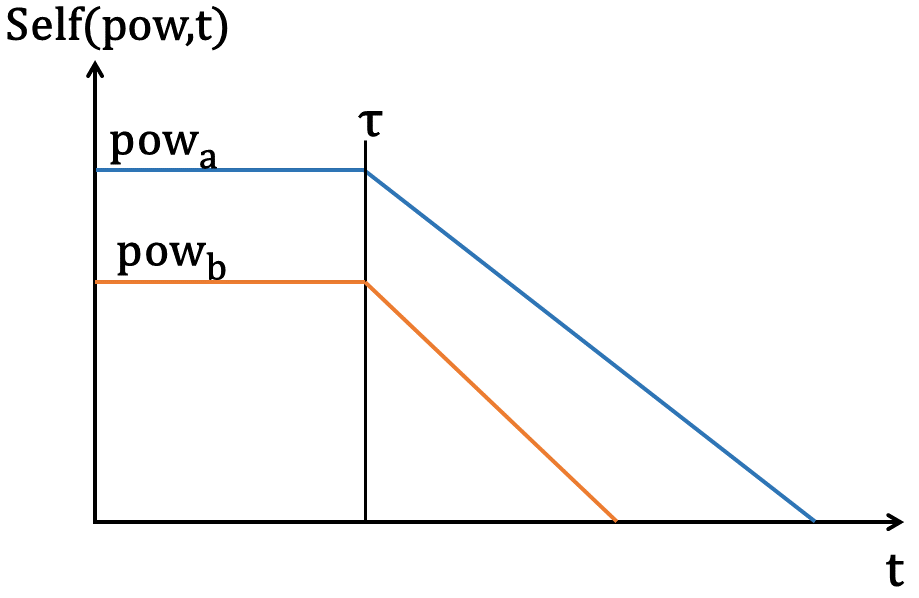
\includegraphics[width=2in]{Figures/chap4/self.png}
			\caption{\label{fig:conc}Courbe de concession reprenant le principe 1}
		\end{figure} 
		
		La fonction $self(dom,t)$ représente le poids que l'agent attribut à sa satisfaction personnelle par rapport à la satisfaction de son partenaire de négociation. Plus la dominance de l'agent est élevée, plus son niveau d'exigence est important. Par ailleurs, la courbe de concession décroît plus rapidement pour des valeurs de dominance faibles.
		
		
	Ces comportements d'exigences et de concessions sont modélisés pour calculer l'acceptabilité d'une proposition 
	
	\subsubsection{Acceptabilité }
	L'acceptabilité d'une valeur de critère $v \in C_i$ est défini comme une fonction booléenne:
	\begin{equation}
	\vspace{0.5em}
	acc(dom,v, t) = sat_{self}(v, \prec_i) \geq  (\beta \cdot self(dom,t))
	\end{equation}
	
	\medskip
	où $\beta>0$ est un paramètre théorique qui définit le poids accordé au niveau d'exigence. Cette fonction est utilisée afin de déterminer si une proposition est acceptable. Par conséquent, nous notons $Ac_i(t) \subseteq C_i $ l'ensemble de valeurs acceptables du critère $C_i$ au moment $t$ de la négociation. 
	
	\begin{equation}
	V_i(dom,t) = \{ v\in C_i : acc(dom,v,t) \}
	\end{equation}
	
	En effet, plus la négociation évolue plus l'agent est apte à faire des concessions. Par conséquent, le nombre de valeurs dans $Ac(t)$ évolue avec le temps. 	Nous notons, donc, $M(t) \not \subseteq Ac(t)$ l'ensemble des valeurs non-satisfaisantes qui peuvent devenir acceptables en raison de concessions: $M(t)=Ac(t)\setminus S$.
	
		\begin{table} [h]
		\centering
		\begin{tabular}{ |c|c|c|c|c| }
			\hline
			value & $ch$ & $jap$ & $it$ & $fr$ \\	
			\hline
			sat(valeur) & 0 & 0.33 & 0.66 & 1 \\
			\hline
		\end{tabular}
		\caption{$Sat$ calculé sur l'ensemble de préférences $\prec_{cuisine}$.}
		\label{tab:ch4sat}	
	\end{table}
	\subsubsection{Exemple}

	Considérons un exemple jouet avec un seul critère de cuisine contenant les valeurs suivantes: 
	$\{$ \emph {français$ (fr)$, italien$ (it)$, japonais$ (jap)$, chinois$ (ch)$}$ \}$. En outre, l'agent a un ordre total de préférences sur ces valeurs$ \prec_ {cuisine}$$ = \{ch$$ \prec$$ jap, jap$$ \prec$$ it,  it$ $\prec$$ fr\}$. Sur la base de cet ordre de préférences $\prec_{cuisine}$, l'agent est capable de calculer la valeur de satisfiabilité associée à chaque valeur comme présenté dans la table \ref {tab:ch4sat}.
	
	
	
	La fonction d'acceptabilité est généralisable aux options $o \in O$:
	 $$acc(dom,o, t) = sat_{self}(o, \prec) \geq  (\beta \cdot self(dom,t))$$

	
	\subsection {Prise en compte des préférences de soi Vs autrui}
	Selon notre second principe, les négociateurs dominants donnent plus de poids à leur propre satisfaction qu'a leur partenaires de négociation. 
	Pour implémenter ce principe dans le contexte de la négociation collaborative, nous calculons dans quelle mesure une proposition donnée est \emph{tolérable} pour la satisfiabilité de l'agent et de son partenaire.
	En effet, à chaque fois que l'agent énoncera une proposition, la valeur de cette dernière doit prendre en compte les préférences des deux interlocuteurs. 
	Donc, pour chaque critère $i\in \mathcal{C}$, considérons le sous ensemble $Ac_i(t)\subseteq C_i$ de valeurs acceptables pour l'agent.
	Cet ensemble correspond à toutes les propositions acceptables qu'un agent pourrait faire à un moment donné de la négociation.
	
	\subsubsection{Tolérabilité}
	Nous calculons la tolérabilité d'une valeur donnée $ v \in Ac_i(t) $ en équilibrant entre les préférences de l'agent et celles de son partenaire. Nous supposons que l'agent donne un poids à la satisfaction de son partenaire qui est complémentaire à son auto-satisfaction:
	
	\begin{equation}
	\begin{split}
	tol(v, t, \prec_i, A_i, U_i, dom) & = self(dom, t)  \cdot sat_{self}(v, \prec_i) \\
	& +  (1 - self(dom, t)) \cdot sat_{other}(v, A_i, U_i)
	\end{split} 
	\end{equation}
	

	Nous généralisons cette fonction à toute option 
	$o = (v_1,\ldots,v_n) \in O$:
	
	\begin{equation}
	tol(o, t, \prec, A, U, dom) = \frac{ \sum_{i}^{n} tol(v_i, t, \prec_i, A_i, U_i, dom) } {n}
	\end{equation}
	
	\noindent
	Par conséquent, l'agent propose la valeur la plus \emph{tolérable} dans l'ensemble $V_i$:
	\begin{equation}
	propose(V_i, \prec_i,dom) =  \operatorname*{arg\,max}_{v \in V_i} ( tol(v))
	\end{equation}
	
	Par conséquent, plus l'agent est soumis, plus il va considérer les préférences de son interlocuteur.
	
	\subsubsection*{Résumé des paramètres computationnels}
	\begin{itemize}[noitemsep]
		
		\item $\pi \in $[0,1] : La frontière entre  les comportements soumis et dominants utilisé dans le choix d'un type d'acte de dialogue.
		\item $\tau > 0$ : le nombre minimal de propositions ouvertes ou rejetées avant le début de la concession.
		\item $\delta > 0$ : paramètre dans la pente de la courbe de concession.
		\item $\alpha> 0$: Le nombre maximums d'actes de dialogues informatifs consécutifs.
	\end{itemize}
	
	\subsection{Contrôle de la négociation}
	\label{chp4:controle}
	
	Le troisième principe stipule que les négociateurs dominants ont tendance à contrôler la négociation.
	Nous avons implémenté ce principe à travers un algorithme pour le choix de l'acte de dialogue à énoncer, comme présenté dans la table \ref{table:uttChoice}.
	
	Nous avons défini un seuil $\pi$  qui divise le spectre de dominance en deux, à savoir comportements dominant, où soumis.
	
	Prenant en compte trois paramètres; la valeur de dominance $dom$, l'acte de dialogue énoncé par le partenaire $u^{-1}$ et l'état courent de la négociation, l'agent sélectionne le premier acte dans la table \ref{table:uttChoice} dont la condition d'applicabilité est vérifiée.  
	
	
	Par exemple, un agent dominant mettra fin à la négociation dès que toutes les options restantes seront inacceptables (ligne 2). Un agent soumis rejettera et exprimera une \emph{State}, afin de justifier son refus et expliquer pourquoi la proposition n'est pas acceptable (ligne 14). S'il n'y a pas de proposition ouverte, l'agent avec une dominance faible demandera de nouvelles informations (ligne 18 -19).
	
	Dans notre modèle, un agent peut exprimer plusieurs actes de dialogues dans un même tour de parole. Ces cas sont représentés avec un signe $"+"$ dans la table \ref{table:uttChoice}.
	
	\begin{table}[!t]
		
		\centering
		\begin{tabular}{|p{.5cm}|p{.9cm}|p{3.6cm}|p{7.6cm}|}
			\hline
			\parbox[t]{3mm}{\multirow{5}{*}{\rotatebox[origin=c]{90}{\centering \textbf{dom  $>\pi$}}}}&$N $de ligne& \textbf{Acte de dialogue} & \textbf{Condition} \\
			\cline{2-4}
			&1&NegotiationSuccess & $\exists o \in T\cup P$, $acc(dom,o,t)$ \\
			\cline{2-4}
			& 2& NegotiationFailure & $ \forall o \in \mathcal{O},  \neg acc(dom,o,t)$\\
			\cline{2-4}
			&3& StateValue(v) & $type(u^{-1}) = AskPreference \land n < \alpha$ \newline $n$ est le nombre d'actes informatifs successifs\\
			\cline{2-4}
			&4& AcceptValue(v)+ \newline ProposeValue(c) & $ \exists v \in P_i$ / $acc(dom,v,t) \land \exists i\in\mathcal{C}, acc(dom,c,t)$ \\
			\cline{2-4}
			&5& AcceptValue(v)+\newline ProposeOption(o) &  $ \exists v \in P_i$ / $ acc(dom,v,t) \land \exists o \in \mathcal{O}$/ $ v \in o \land acc(dom,o,t)$ \\
			\cline{2-4}
			&6& RejectValue(v)+\newline ProposeValue(c) & $ \exists v \in P_i$ / $ \neg acc(dom,v,t) \land \exists i\in\mathcal{C}, acc(dom,c,t)$ \\
			\cline{2-4}
			&7& RejectValue(v)+ \newline ProposeOption(o) &  $ \exists v \in P_i$ / $  \neg acc(dom,v,t) \land \exists o \in \mathcal{O}$/ $acc(dom,o,t)$ \\
			\cline{2-4}
			& 8&RejectOption($o_1$)+ ProposeOption($o_2$) & $ \exists o_1 \in P$ / $ \neg acc(dom,o_1,t) \land \exists o_2\in\mathcal{O}, acc(dom,o_2,t)$ \\
			\cline{2-4}
			&9& ProposeValue(v) & $\exists v \in C_i$ / $tol(v, t, \prec_i, A_i, U_i, dom)$\\
			\cline{2-4}
			&10& ProposeOption(o) & $\exists o \in \mathcal{O}$ / $tol(o, t, \prec_i, A_i, U_i, dom)$\\
			
			\hline
			
			\parbox[t]{2mm}{
				\multirow{5}{*}{\rotatebox[origin=c]{90}{ \textbf{dom  $ \leq \pi$}}}} & 11& Negotiation success &  $\exists o \in T$ \\
			\cline{2-4}
			&12& AcceptValue(v) & $\exists i\in\mathcal{C}, \exists v \in P_i, acc(dom, v, t)$ \\
			\cline{2-4}
			&13&AcceptOption(o) & $\exists o \in P, acc(dom, o, t)$ \\
			\cline{2-4}
			&14&RejectValue(v)+\newline StateValue(v) & $ t<\tau \land (\exists i\in\mathcal{C}, \exists v \in P_i, \neg acc(dom,v, t))$.\\
			\cline{2-4}
			&15&RejectOption(o)+ \newline StateValue(v) & $ t<\tau \land (\exists o \in P,  \neg acc(dom,o, t) \land \exists v \in o, \neg acc(dom,v, t))$.\\
			\cline{2-4}
			&16&ProposeValue(v) &  $\exists i\in\mathcal{C}, \exists v \in C_i, v \in A_i  \land acc(dom, v, t) $\\
			\cline{2-4} 
			&17&ProposeOption(o)  & $\forall i\in\mathcal{C},\exists v \in C_i, v \in T_i  \land v \in o$ \\
			\cline{2-4} 
			&18&AskValue(v) & $t > \tau \land \exists i\in\mathcal{C}, \exists c \in P_i, \neg acc(c, t)$ \\
			\cline{2-4} 	
			&19&AskCriterion(i) & $\exists i\in\mathcal{C}, A_i \cup U_i= \emptyset $\\
			\cline{2-4}	
			&20&StateValue(v) & $\exists i\in\mathcal{C}, C_i\cap S_i \neq \emptyset$	\\
			\cline{2-4}
			&21& ProposeValue(v) & $\exists v \in C_i$ / $tol(v, t, \prec_i, A_i, U_i, dom)$\\
			\cline{2-4}
			&22& ProposeOption(o) & $\exists o \in \mathcal{O}$ / $tol(o, t, \prec_i, A_i, U_i, dom)$\\
			
			\hline
		\end{tabular}
		
		\caption{Ordre de sélection d'actes de dialogues en fonction de la valeur de dominance}
		\label{table:uttChoice}
	\end{table}
	
	En fonction de la valeur de dominance, l'agent va adopter différentes stratégies dans la sélection de l'acte de dialogue à exprimer. En effet, dans les travaux en psychologie social, les négociateurs dominants se concentrent sur l'avancement de la tâche de négociation. Ceci ce traduit par le choix d'actes de négociations (ProposeValue /ProposeOption, RejectValue /RejectOption, AcceptValue/ AcceptOption) comme il est présenté dans les lignes (4 à 10).
	
	L'agent priorise les actes de négociations plutôt que les actes d'échanger d'informations sur les préférences. En effet, comme présenté à la ligne 3, après un nombre de tours $ \alpha $ consacrés au partage d'informations, l'agent fera plutôt des propositions que informer le partenaire de ses goûts. Un exemple est présenté dans le dialogue \ref{fig: ex-dialogue}.
	
	Au contraire, un négociateur soumis se concentrera sur la construction d'un modèle précis des préférences de son partenaire afin de prendre la décision la plus équitable. Il se concentrera plus sur \emph {actes d'échanges d'information} (StateValue ou AskValue / AskCriterion) comme le montre les lignes (18-20). De plus, les mouvements de négociation sont limités par des conditions qui garantissent que l'agent ait rassemblé suffisamment d'informations sur les préférences de son partenaire avant d'exprimer une proposition (ligne 16-17).
	
	
	
	\begin{figure*}[!t]
	\begin{minipage}{\textwidth}
			{\ttfamily
				\begin{addmargin}[1em]{2em}% 1em left, 2em right
					\vspace{0.5 em}
					1. \textbf{A:} $Propose(eiffel\_tower)$ "Let's go to a restaurant near \hspace*{3mm} eiffel tower."
					
					
					2. \hspace*{3mm}\textbf{B}: $RejectState(eiffel\_tower)$ "I don't like restaurants \hspace*{4mm} near eiffel tower, let's choose something else."
					
					
					3. \textbf{A:} $Propose(Ebis)$ "Let's go to the Ebis restaurant. It's \hspace*{3mm} a lively, expensive Japanese restaurant on the near \hspace*{3mm} eiffel tower."
					
					
					4. \hspace*{3mm}\textbf{B}: $AskPreference(Montparnasse)$ "Do you like \hspace*{4mm} restaurants at montparnasse?"
					
					
					5. \textbf{A}: $StatePreference(Montparnasse,false)$ "I don't like \hspace*{3mm} restaurants at montparnasse."
					
					
					6. \hspace*{3mm}\textbf{B}: $AskPreference(Gare\_du\_nord)$ "Do you like restaurants \hspace*{4mm} at gare du nord?"
					
					
					7. \textbf{A}: $Propose(Ebis)$ "Let's go to the Ebis restaurant. It's \hspace*{3mm} a lively, expensive Japanese restaurant on the near \hspace*{3mm} eiffel tower."
					
					
					8. \hspace*{3mm}\textbf{B}: $AskPreference(Gare\_du_nord)$ "Do you like restaurants \hspace*{4mm} at gare du nord?"
					
					
					9. \textbf{A}: $StatePreference(Gare\_du\_nord,false)$ "I don't like \hspace*{3mm} restaurants at gare du nord."
					
					
					10. \hspace*{3mm}\textbf{B}: $AskPreference(pere\_lachaise)$ "Do you like restaurants \hspace*{4mm} at pere lachaise?"
					
					
					11. \textbf{A}: $Propose(cozy)$ "Let's go to a cozy restaurant."
					
					
					12. \hspace*{3mm}\textbf{B}: $Accept(cozy)$ "Okay, let's go to a cozy \hspace*{4mm} restaurant."
					
					
					13. \textbf{A}: $Propose(expensive)$ "Let's go to an expensive \hspace*{3mm} restaurant."
					
					
					14. \hspace*{3mm}\textbf{B}: $Accept(expensive)$ "Okay, let's go to an expensive \hspace*{4mm} restaurant."
					
					
					15. \textbf{A}: $Propose(Juji)$ "Let's go to the Juji restaurant. It's a \hspace*{3mm} cozy, expensive Japanese restaurant on the near \hspace*{3mm} eiffel tower."
					
					
					16. \hspace*{3mm}\textbf{B}: $Accept(Juji)$ "Okay, let's go to the Juji \hspace*{4mm} restaurant."
					\vspace{0.5 em}
				\end{addmargin}
			}
	\end{minipage}
			\caption{\label{fig: ex-dialogue} Exemple de dialogue généré avec un agent A $dom_A$ = 0.8 et un agent B $dom_B$ = 0.4}
\end{figure*}
	
	\section{Évaluation du modèle}
		
		Dans cette section, nous présentons une première évaluation de notre modèle de négociation collaborative. Cette dernière a pour objectif de valider l'implémentation de notre modèle de négociation collaborative et d'étudier la perception des comportements de dominance exprimés par l'agent au cours d'une négociation. 
		Pour ce faire, nous avons mené deux études, la première étude agent/agent où les participants avaient le rôle de juge externe pour évaluer le comportement des agents lors de leur négociation.
		La seconde étude visait à évaluer les comportements de l'agent au cours d'une interaction avec un utilisateur humain. Par conséquent, les participants ont négocié avec des agents pour ensuite évaluer leurs comportements. 
		
		\subsection{Hypothèses}
				
				Nous avons défini quatre hypothèses qui reflètent les différents comportements et stratégies affichés par les agents lors de la négociation. Dans ce qui suit, nous noterons l'agent qui exhibe des comportements dominants dans la relation interpersonnelle comme \emph{agent dominant}, et l'agent dans la position soumise comme \emph{l'agent soumis}.
				
				\begin{itemize}
					\item \textbf {H1:} L'agent dominant sera plus fortement perçu comme étant égocentrique que l'agent soumis.
					
					\item \textbf {H2:} L'agent dominant sera plus fortement perçu comme exigeant que l'agent soumis.
					
					\item \textbf {H3:} L'agent soumis sera perçu comme faisant des concessions plus importantes que l'agent dominant.
					
					\item \textbf {H4:} L'agent dominant sera plus fortement perçu comme prenant le contrôle de la négociation que l'agent soumis.
					
				\end{itemize}
				
				Ces hypothèses sont utilisés pour valider les comportements de dominance de nos agents négociateurs dans les deux études. 
				
		\subsection{Étude 1: Évaluation Agent/Agent}
				L'objectif de cette étude est d'analyser la perception des différents comportements de dominance qui peuvent apparaître au cours d'une négociation. En effet, chaque comportement implémenté est lié à un principe et donc indépendant des autres principe. Nous visons donc à étudier si les différents comportements de l'agent durant la négociation vont être correctement associé à des comportements de dominance. Pour ce faire, nous avons généré des dialogues entre deux agents doté de notre modèle de négociation. 
			
			\subsubsection{Implémentation des agents négociateurs}
				Nous avons implémenté deux agents qui devaient simuler une relation interpersonnelle de dominance. Pour ce faire, un agent a été initialisé pour produire des comportements dominants et l'autre agent produisait des comportements complémentaire de soumission. 
				
				
				Nous avons manipulé des paramètres de simulations afin d'initialiser les comportements des deux agents.
				
				\paragraph{i. Variables comportementales}
				
				Premièrement, nous avons fixé les paramètres computationnels de nos fonctions de décisions: $\tau=2$, $\pi=0.5$, $\alpha=2$, $\beta=1$ et $\delta=0.1$. 
				Deuxièmement, nous avons choisi les valeurs de dominance $dom$ de chaque agent afin de le positionner dans le spectre de dominance. 
				Ensuite, nous avons défini les préférences de chaque agent. En effet, les préférences ont un impact direct sur le processus de décision, il fallait donc générer des préférences différentes qui vont stimuler le processus de décision. Pour cela, nous avons utilisé la mesure de distance \emph{Kendall tau} \cite{bra2013Kendall} qui permet de calculer la distance entre deux ensembles de préférences d'ordre partiel. 
				Nous présentons dans ce qui suit la définition de la distance de Kendall. 
				
				\vspace{1 em}
				\paragraph{ii. Distance de Kendall}
%				\vspace{0.75 em}
				La distance de \emph{Kendall} considère les distances entre deux ordres partiels en fonction de leurs ensembles d'extensions totales.
				
				Pour chaque ensemble partiel, l'algorithme génère des extensions de cet ensemble jusqu'à arriver à un des ordre total. Pour un ensemble $\sigma$, nous notons l'ensemble des extensions possibles de ce modèle $ext(\sigma)$.
				
				La distance entre deux modèle partiels  $\sigma$ et $\mu$ est donc calculé comme suit: 

				
				\begin{equation*}
					K_H(\sigma,\mu) = max \left \{ \max\limits_{\alpha \in ext(\sigma)} \min\limits_{\beta \in ext(\mu)} K(\alpha , \beta), \max\limits_{\beta \in ext(\mu)} \min\limits_{\alpha \in ext(\sigma)} K(\beta, \alpha)  \right \}
				\end{equation*}
				
				tel que $K(\alpha , \beta)$ est la distance entre les deux ensembles d'ordre totaux $\alpha$ et $\beta$ qui compte le nombre les désaccords ou des inversions de paires de préférences entre les deux ensembles. 
				 
				\paragraph{iii. Domaine de négociation}
				
				Enfin, nous avons défini le sujet de négociation. Nous avons opté pour un sujet social qui n'exige pas de compétence techniques. Les négociateurs avait pour but de négocier afin de choisir un restaurant. Nous avons pris en compte quatre critères pour le choix d'un restaurant. 	Les critères sélectionnés sont \ {\textit {cuisine, prix, ambiance, emplacement} \}. Chaque critère a été défini avec un domaine de valeurs, et un total de 420 restaurants a été généré à partir des valeurs de chaque critère.
				
				Afin d'analyser la perception des comportements de dominances des agents, il faut varier les paramètres d'initialisation des agents, à savoir la valeur de dominance ainsi que les préférences
				
				La variation de ces comportements définit nos conditions expérimentales. 
				Au total, nous avons généré quatre conditions expérimentales résumées dans la table \ref{table:conditions}. 
				
				Nous avons généré un dialogue par condition pour un total de 4 dialogues: trois dialogues avec des agents dont les préférences sont distantes. Un seul dialogue a été produit pour la condition dans laquelle les préférences des agents sont similaires. En effet, quand les préférences sont similaires les dialogues générés se ressemblaient et convergeaient rapidement vers un compromis. Par conséquent, les comportements produits étaient proches même en variant la valeur de dominance initiale de l'agent.   
				
				Les dialogues générés sont disponibles en annexe \ref{annexe:crowd}.
				
				\begin{table}[h]
					\centering
					\begin{tabular}{ |l|c|c|l| }
						\hline
						\textbf{Préférences}& \textbf{A} & \textbf{B} & \textbf{Label} \\ 
						\hline
						\newline\multirow{3}{*} {Préférences distantes (Kendall's tau = $0.96$)} & 0.9 & 0.4 & Dialogue 1 \\ \cline{2-4}
						
						\newline  & 0.7 & 0.4 & Dialogue 2\\ \cline{2-4}
						
						\newline   &0.7 & 0.2 & Dialogue 3\\ 
						\hline
						\newline Préférences similaire (Kendall's tau = $0.46$) & 0.7 & 0.4 & Dialogue 4\\
						\hline
					\end{tabular}
					\caption{Conditions expérimentales pour la génération des dialogues.} 
					\label{table:conditions}
				\end{table}
		
			\subsubsection{Procédure}
					\label{sec:questionnaire}
					Nous avons mené une étude inter-sujets via le site web de crowdsourcing  \emph {CrowdFlower} \footnote {https://www.crowdflower.com/}.
					Chaque participant a évalué uniquement un seul dialogue pour lequel les agents A et B étaient décrits comme deux amis essayant de négocier un restaurant pour dîner.
					Les participants ont été invités à lire le dialogue qui leur a été assigné et à répondre à un questionnaire.
					Deux questions ont été défini pour chaque hypothèse. Par ailleurs, nous avons inclus deux questions de test pour vérifier la crédibilité des réponses fournies par les participants. Par la suite, nous avons écarté les participants ayant fourni des mauvaises réponses à ces questions. 
					Chaque item devait être évalué sur une échelle de Likert à 5 points allant de ``Je ne suis pas du tout d'accord'' à ``Je suis totalement d'accord".
			
					Les items du questionnaires sont présentés dans la table \ref{table:questionnaire}. L'étude ayant été réalisé sur une population anglophone, nous présentons les questions dans leurs version originale. 
						
								\begin{table}[h]
																\centering
								\begin{tabular}{|p{1.75cm}|p{4cm}|p{4.8cm}|}

									\hline
									Hypothesis &question 1& question 2 \\
									\hline
									\textbf{H1} &Speaker (A/B) is self-centered. &Speaker (A/B) takes his friend's preferences into account in the choice of the restaurant.\\
									\hline
									\textbf{H2} &Speaker (A/B) makes concessions in the negotiation.&Speaker (A/B) gives up his position in the negotiation\\
									\hline
									\textbf{H3} & Speaker (A/B) is demanding&Speaker (A/B) presses his position in the negotiation. \\
									\hline
									\textbf{H4} &Speaker (A/B) takes the lead in the negotiation.&Speaker (A/B) takes the initiative in the negotiation \\
									\hline
								\end{tabular}
							
							\caption{Items proposés pour le questionnaire sur la perception des comportements de dominance.}
							\label{table:questionnaire}
						\end{table}
					
					Au total 120 participants ont pris part à l'étude (30 par condition). Les participants devaient être anglophone de naissance. Chaque sujet a perçu \textit{25 cents} pour sa participation. Au final, 15 participants ont été exclus pour avoir mal répondu au questions de test. 
					
					Dans la prochaine section, nous présentons l'analyse des donnés obtenus suite à cette étude.
					
					
			\subsubsection{Résultats}
				Comme nous avions formulé deux questions pour chaque hypothèse, nous avons d'abord calculé la corrélation entre chaque paire de question. En moyenne, nous avons obtenus une corrélation de l'ordre de $0.5$. Cette forte corrélation nous permet d'utiliser ces données pour évaluer les comportements des locuteurs (speakers) sur chaque principe. 
				
				L'ensemble des résultats sont résumés dans la table \ref{tab:resetude1}. Nous avons commencé par effectuer les statistiques descriptives pour évaluer la perception des comportements de dominance affilié à chaque agent. 
					\begin{itemize}
							\item \textbf{Soi versus autrui :} L'agent A qui exprimait des comportements de dominance a été en moyenne vu comme égocentrique, alors que l'agent B, l'agent soumis, n'a pas été vu comme égocentrique et ce résultat a été trouvé pour les quatre dialogues.
							Par exemple, pour le dialogue 2, l'agentA a été moyenne perçu comme s'intéressant uniquement à ses préférences \textit{(M=3.6, ET=0.9)} contrairement à l'agent B \textit{(M=2.2, ET=0.8)}.
							
							\item \textbf{Niveau exigence et concessions :} En moyenne l'agent A a été perçu comme exigent durant le dialogue. Par exemple, les participants ayant évalué le dialogue 1 ont trouvé que l'agent A était exigent \textit{(M=4.1, ET=0.8)} alors que l'agent B n'a pas du tout été perçu comme exigent durant la négociation \textit{(M=2.6, ET=1.1)}. A l'opposé, l'agent B a été vu comme exprimant des concessions durant la négociation contrairement à l'agent A. Par exemple, dans le dialogue 1, l'agent A été perçu comme n'exprimant que trés peu de concessions \textit{(M=2.2, ET=1.1)} contrairement à l'agent B qui a été largement évalué comme exprimant des concessions \textit{(M=4.3, ET=0.8)}.
							
							\item  \textbf{Le contrôle de la négociation:} Les comportements de prise de contrôle ont été correctement perçu par les participants. En effet, même dans le condition ou les préférences des agents étaient similaires dont le dialogue était assez court, les participants ont perçu l'agent A comme leader de la négociation \textit{(M=4.5, ET=0.9)}, tandis que l'agent B a été en moyenne perçu comme manquant de prise d'initiatives \textit{(M=1.9, ET=0.9)}.
					\end{itemize}
				
			Nous avons ensuite comparé les comportements des deux agents pour chaque principe. Pour ce faire, nous avons en premier lieu analysé la distribution des données qui nous a révélé que ces dernières ne suivent pas une distribution normale. C'est la raison pour laquelle nous avons utilisé un test non-paramétrique de \emph{Wilcoxon  de rang signé} afin de comparer la perception des comportements de l'agent A contre l'agent B.
			
			Les résultats présentés dans la figure \ref{fig:H1} montrent que l'agent A qui produisait des comportements dominant a été largement perçu comme étant plus centré sur lui-même, comme supposé par l'hypothèse \textbf {H1}, avec une taille d'effet importante. Par exemple, considérons le dialogue 1 sur la Table~\ref {tab:resetude1}, le test statistique indique que l'agent A était significativement perçu comme étant plus centré sur lui-même que l'agent B avec (\emph {Z = -5.28} et  \emph {p $ <0,001 $}).
			
			Par ailleurs, une différence significative dans le niveau des concessions exprimé dans tous les dialogues a été révélée confirmant notre hypothèse \textbf {H2}. En effet, les résultats dans la figure \ref{fig:H2} montrent que l'agent dominant était perçu comme faisant moins de concessions. La taille d'effet a montré un effet moyen pour les dialogues 2 à 4, et un effet important pour Dialogue 1 avec (\emph {Z = -5.34} et \emph {p $ <$ 0.001}).
			
			L'hypothèse \textbf {H3} a également été confirmée par le \emph {test de rang signé de Wilcoxon} (voir figure \ref{fig:H3}), où l'agent A a été perçu comme le négociateur le plus exigeant, avec une grande taille d'effet observée pour tous les dialogues. 
			
			L'hypothèse (\textbf {H4}) a été confirmée. Le test de Wilcoxon a révélé que l'agent A avec des comportements dominants  était perçu comme significativement plus leader du dialogue que l'agent B, avec une grande taille d'effet pour les dialogues 1, 2 et 4, et une taille d'effet moyenne pour le dialogue3 comme décrit dans Table~\ref {tab:resetude1} et la figure \ref{fig:H4}.

				
				\begin{figure}[!htb]
					\subfloat[Résultats pour l'hypothèse H1 sur l'égocentrisme \label{fig:H1}]{%
						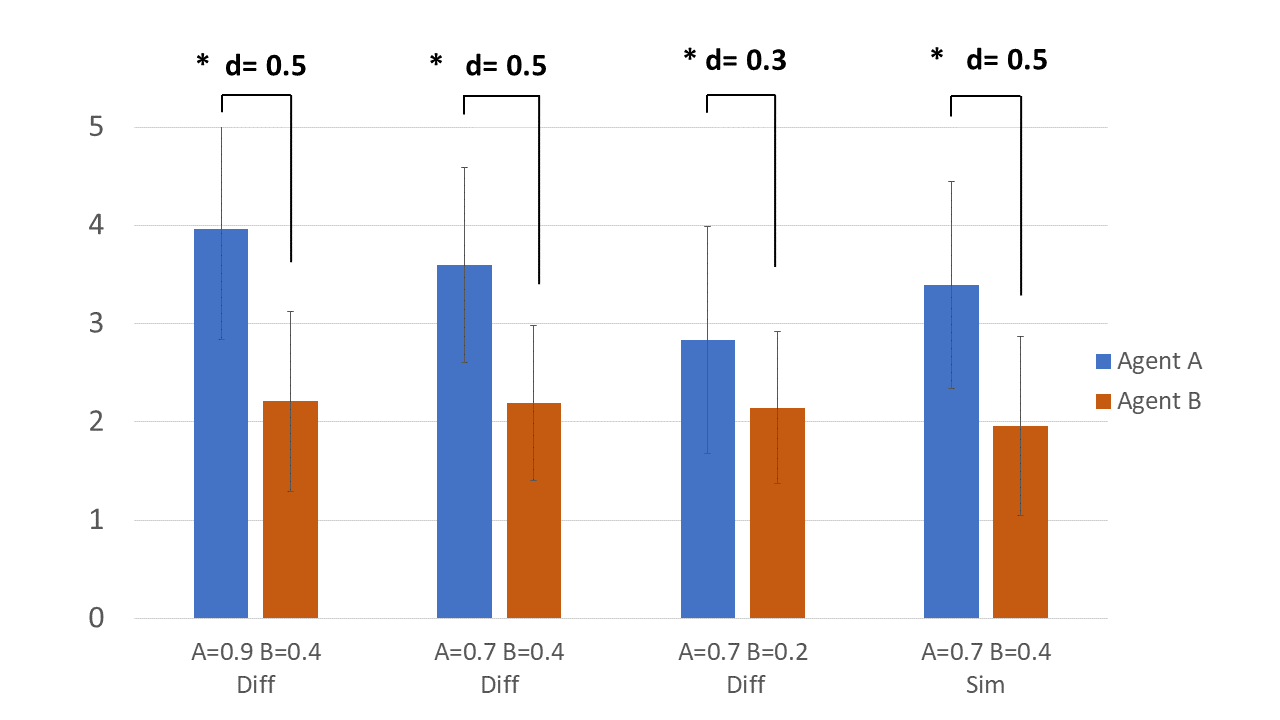
\includegraphics[width=0.48\textwidth]{Figures/chap4/AA/graphs/Diapositive1.PNG}
					}
					\hfill
					\subfloat[Résultats pour l'hypothèse H2 sur le niveau de concessions \label{fig:H2}]{%
						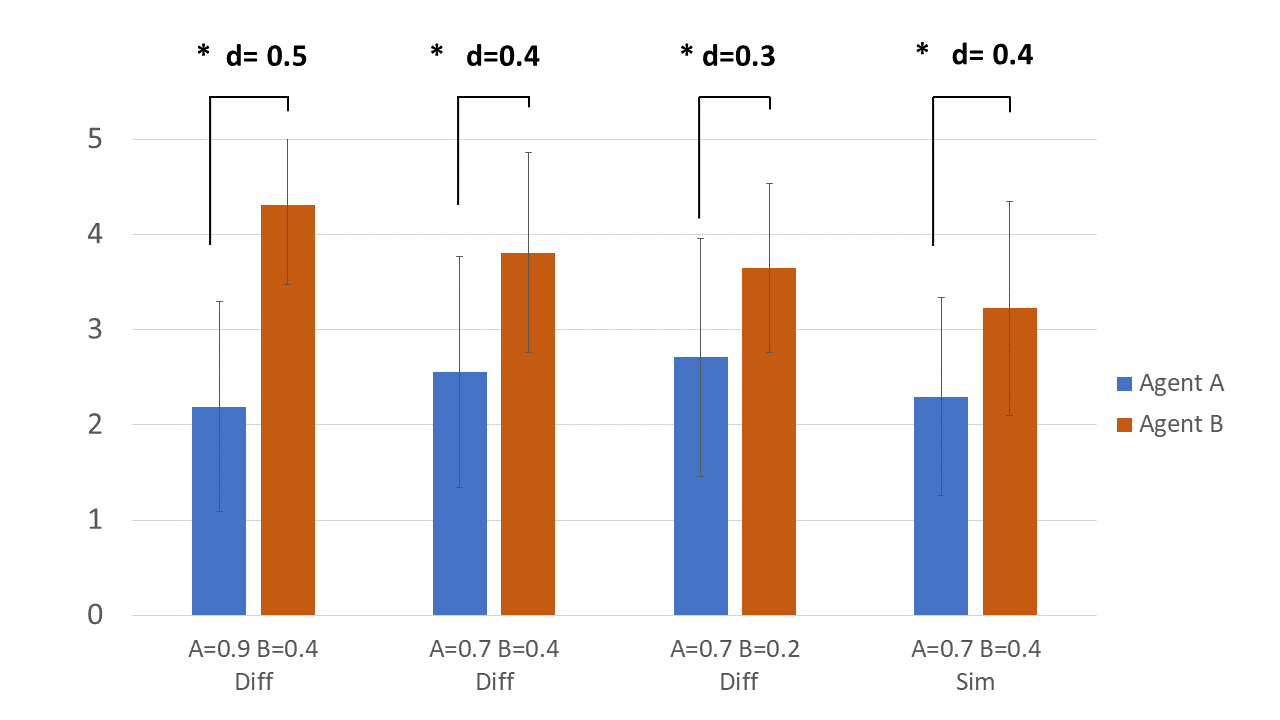
\includegraphics[width=0.48\textwidth]{Figures/chap4/AA/graphs/Diapositive2.PNG}
					}
					
					\caption{Résultats statistiques}
				\end{figure}
				
			   \begin{figure}[!htb]
			   	
			   	\subfloat[Résultats pour l'hypothèse H3 sur le niveau d'exigence\label{fig:H3}]{%
			   		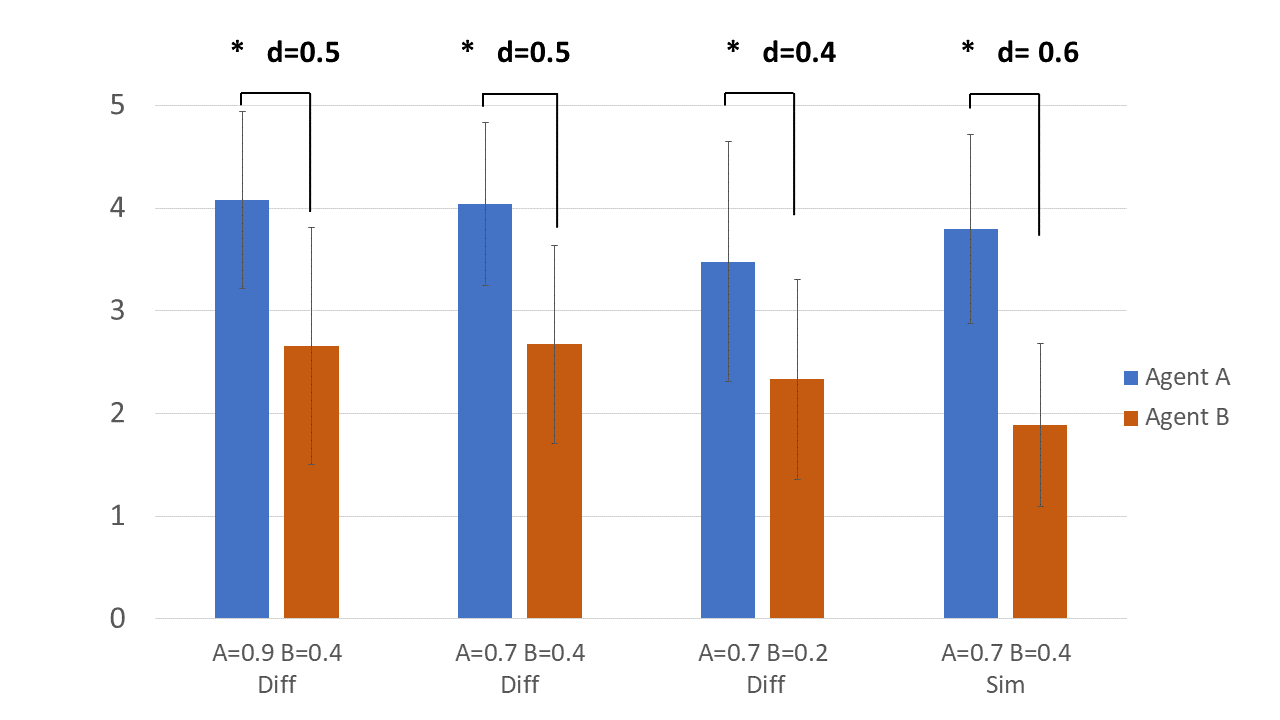
\includegraphics[width=0.48\textwidth]{Figures/chap4/AA/graphs/Diapositive3.PNG}
			   	}
		   		\hfill
		   		\subfloat[Résultats pour l'hypothèse H4 sur la prise de contrôle \label{fig:H4}]{%
		   			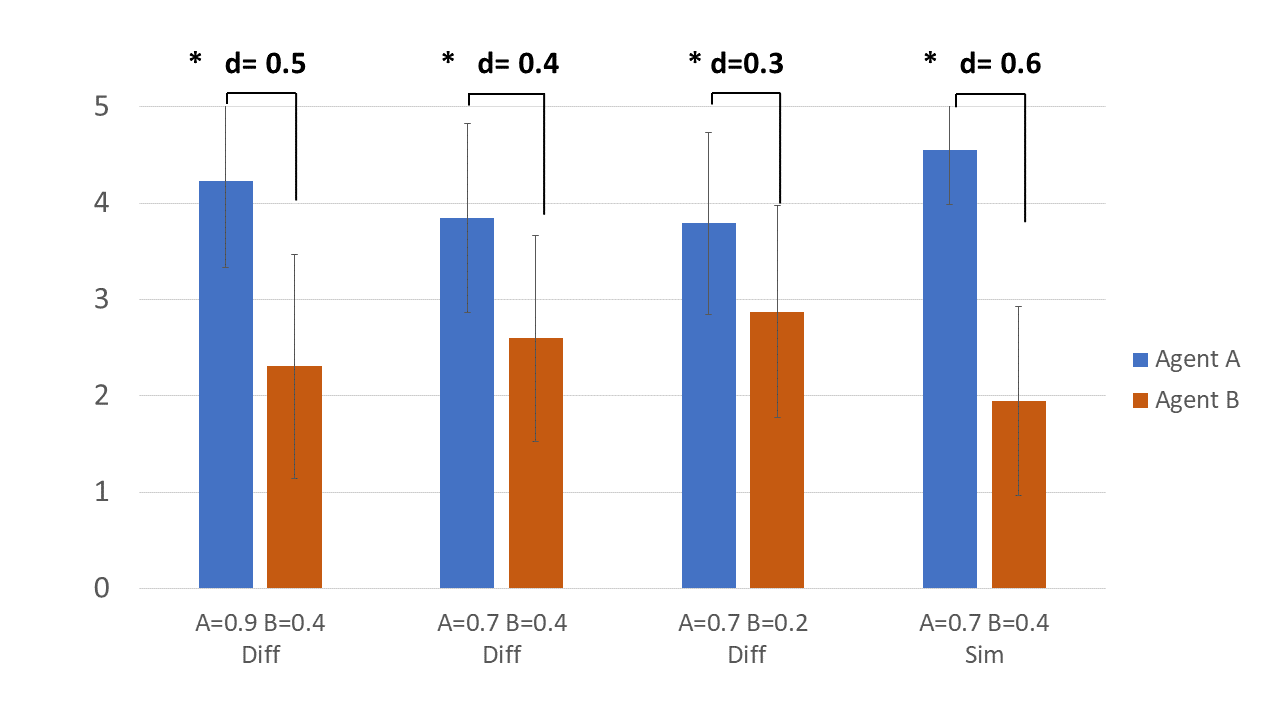
\includegraphics[width=0.48\textwidth]{Figures/chap4/AA/graphs/Diapositive4.PNG}
		   		}
				  \caption{Résultats statistiques}
			   	\end{figure}

				   
				   
	
			
		\begin{table*}
				\begin{adjustbox}{angle=90}
					\begin{tabular}{|ll|c|c|c|c|c|c|c|c|} 
						\cline{3-10}
						
						\multicolumn{1}{c} {}	& \multirow{2}{*} {}& \multicolumn{2}{c|} {Dialogue1} & \multicolumn{2}{c|} {Dialogue2} & \multicolumn{2}{c|} {Dialogue3} &\multicolumn{2}{c|} {Dialogue4} \\ 
						\cline{3-10}
						
						
						\multicolumn{1}{c} {} & & SpeakerA & SpeakerB & SpeakerA & SpeakerB & SpeakerA & SpeakerB & SpeakerA & SpeakerB \\
						\hline 
						%\multicolumn{9}{|c|}{ \textbf{Results for H1}} \\
						%	\hline
						\newline \multirow{4}{*} {\textbf{H1}}  & \multicolumn{1}{|l|}{ \textit{Moyenne} $\pm$ \textit{ET} } & 3.9 $\pm$ 1.1 & 2.2$\pm$ 0.9  & 3.6 $\pm$0.9 & 2.2 $\pm$0.8  &2.8 $\pm$1.1  & 2.13$\pm$ 0.7 & 3.4 $\pm$ 1 & 2 $\pm$0.9 \\
						\cline{2-10}	
						\newline & \multicolumn{1}{|l|}{p-value} & \multicolumn{2}{c|}{ $9.75E^{-08}$} & \multicolumn{2}{c|}{ $5.14E^{-08}$} & \multicolumn{2}{c|}{ $0.002$}& \multicolumn{2}{c|}{ $6.23E^{-08}$}\\
						\cline{2-10}	
						% -------------
						\newline & \multicolumn{1}{|l|}{Z-Wilcoxon test} & \multicolumn{2}{c|}{ $-5.28$} & \multicolumn{2}{c|}{ $-5.34$} & \multicolumn{2}{c|}{ $-3$}& \multicolumn{2}{c|}{ $-4.93$}\\
						\cline{2-10}	
						%*************
						\newline & \multicolumn{1}{|l|}{Taille d'effet (d)} & \multicolumn{2}{c|}{ $0.51$} & \multicolumn{2}{c|}{ $0.52$} & \multicolumn{2}{c|}{ $0.3$}& \multicolumn{2}{c|}{ $0.47$}\\
						\hline	
						%*************
						
						\newline \multirow{4}{*} {\textbf{H2}} &\multicolumn{1}{|l|}{ \textit{Moyenne} $\pm$ \textit{ET} } & 2.2 $\pm$ 1.1 & 4.3$\pm$ 0.8  & 2.5 $\pm$1.2 & 3.8 $\pm$1.04 &2.7 $\pm$1.2  & 3.6$\pm$ 0.8 & 2.3 $\pm$ 1 & 3.2 $\pm$1.2 \\
						\cline{2-10}	
						\newline & \multicolumn{1}{|l|}{p-value} & \multicolumn{2}{c|}{ $7.07E^{-08}$} & \multicolumn{2}{c|}{ $3.71E^{-05}$} & \multicolumn{2}{c|}{ $=0.01$}& \multicolumn{2}{c|}{ $1.73E^{-04}$}\\
						\cline{2-10}	
						
						% -------------
						\newline & \multicolumn{1}{|l|}{Z-Wilcoxon test} & \multicolumn{2}{c|}{ $-5.34$} & \multicolumn{2}{c|}{ $-4.05$} & \multicolumn{2}{c|}{ $-3.13$}& \multicolumn{2}{c|}{ $-3.69$}\\
						\cline{2-10}	
						%*************
						\newline & \multicolumn{1}{|l|}{Taille d'effet (d)} & \multicolumn{2}{c|}{ $0.52$} & \multicolumn{2}{c|}{ $0.39$} & \multicolumn{2}{c|}{ $0.32$}& \multicolumn{2}{c|}{ $0.35$}\\
						\hline	
						%*************
						
						\newline \multirow{4}{*} {\textbf{H3}} &\multicolumn{1}{|l|}{ \textit{Moyenne} $\pm$ \textit{ET} } & 4.1 $\pm$ 0.8 & 2.6$\pm$ 1.1 & 4.03 $\pm$ 0.8 & 2.7 $\pm$0.9 &3.5 $\pm$1.1 & 2.3$\pm$ 1 & 3.8 $\pm$ 1.8 & 1.8 $\pm$0.8 \\
						\cline{2-10}	
						\newline & \multicolumn{1}{|l|}{p-value}  & \multicolumn{2}{c|}{ $2.93E^{-08}$} & \multicolumn{2}{c|}{ $4.77E^{-07}$} & \multicolumn{2}{c|}{ $1.19E^{-04}$}& \multicolumn{2}{c|}{ $2.56E^{-09}$}\\
						\cline{2-10}	
						%				
						% -------------
						\newline & \multicolumn{1}{|l|}{Z-Wilcoxon test} & \multicolumn{2}{c|}{ $-4.62$} & \multicolumn{2}{c|}{ $-4.96$} & \multicolumn{2}{c|}{ $-3.80$}& \multicolumn{2}{c|}{ $-5.86$}\\
						\cline{2-10}	
						%*************
						\newline & \multicolumn{1}{|l|}{Taille d'effet (d)} & \multicolumn{2}{c|}{ $0.45$} & \multicolumn{2}{c|}{ $0.49$} & \multicolumn{2}{c|}{ $0.39$}& \multicolumn{2}{c|}{ $0.56$}\\
						\hline	
						%*************
						
						\newline \multirow{4}{*} {\textbf{H4}} & \multicolumn{1}{|l|}{ \textit{Moyenne} $\pm$ \textit{SD} } & 4.2 $\pm$ 0.9 & 2.3$\pm$ 1.1  & 3.8 $\pm$0.9 & 2.6 $\pm$1.07 & 3.8 $\pm$0.9  & 2.8$\pm$ 1.1  & 4.5 $\pm$0.5  & 1.9 $\pm$ 0.9\\
						\cline{2-10}
						\newline & \multicolumn{1}{|l|}{p-value} & \multicolumn{2}{c|}{ $2.44E^{-07}$} & \multicolumn{2}{c|}{ $3.28E^{-05}$} & \multicolumn{2}{c|}{ $0.03$}& \multicolumn{2}{c|}{ $7.04E^{-10}$}\\
						\cline{2-10}	
						% -------------
						\newline & \multicolumn{1}{|l|}{Z-Wilcoxon test} & \multicolumn{2}{c|}{ $-5.11$} & \multicolumn{2}{c|}{ $-4.08$} & \multicolumn{2}{c|}{ $-2.86$}& \multicolumn{2}{c|}{ $-6.09$}\\
						\cline{2-10}	
						%*************
						\newline & \multicolumn{1}{|l|}{Taille d'effet (d)} & \multicolumn{2}{c|}{ $0.5$} & \multicolumn{2}{c|}{ $0.4$} & \multicolumn{2}{c|}{ $0.29$}& \multicolumn{2}{c|}{ $0.57$}\\
						\hline	
						%*************
					\end{tabular}
					
					\caption{Résumé des résultats statistiques obtenus pour chaque hypothèses}
					\label{tab:resetude1}
				\end{adjustbox}
			\end{table*}
				
			\subsubsection{Discussion}	
				Dans cette étude, nous avons présenté des dialogues générés entre deux agents négociateurs simulant une relation interpersonnelle de dominance. 
				Les résultats obtenus confirment l'ensemble de nos hypothèses. En effet, l'analyse de ces dialogues par des juges externes a révélé que ces derniers étaient en mesure de percevoir les comportements de dominance exprimés par les deux agents. L'agent A qui était placé dans la position dominante a été perçu comme plus égocentrique, exigeant, leader et exprimait peu de concessions durant la négociation. En revanche, l'agent B qui exprimait des comportements de faible dominance (soumission) a été perçu comme prenant en compte les préférences de son interlocuteur, peu exigent, avait tendance à faire des concessions mais ne prenait pas assez d'initiatives.  
				
				Par ailleurs, nous avons réalisé une analyse post-étude qui avait pour but de comparer la perception des comportements de l'agent A à travers les différents dialogues. 
				Nous avons calculé la différence entre l'évaluation de l'agent A et B dans le dialogue 1 et le dialogue 2. En effet, dans le dialogue 1 l'agent A a une dominance à 0.9, alors que dans le dialogue 2, sa dominance est à 0.7. En revanche, la position de dominance de l'agent B est fixée à 0.4 pour les deux dialogues. 
				
				Notre hypothèse était qu'une plus grande différence de dominance entre les interlocuteurs conduirait à une meilleure perception de leurs comportements. Les résultats obtenus ne confirment pas cette hypothèse. En effet, seulement une tendance a été observée ($ p \simeq 0,1 $) pour l'égocentrisme, les concessions et le niveau d'exigence. Seule une corrélation entre la dominance et la prise de contrôle de la négociation était nettement perçu ($p = 0.043$). Plus la position de dominance de l'agent augmentait, plus il était perçu comme leader. 
				
				Ces résultats mitigés renforcent la définition dyadique de la dominance. La perception des comportements de dominance d'un interlocuteur est relative à ceux exprimés par son partenaire \cite{dunbar2005perceptions}. 
				Pour cette raison, agréger les évaluations des différents dialogues n'apporte pas d'informations pertinente. Ceci explique pourquoi nous avons obtenu des résultats mitigés sur cet aspect.
				
				Une limite de cette étude que nous avons étudié la perception de tous les principes liés à la dominance simultanément. Nous n'avons pas considéré la perception de chaque principe individuellement. Cependant, lors des expériences précédentes, nous avons détecté que les principes sont interdépendants, ce qui rend difficile une évaluation séparée de chacun d'entre eux dans un dialogue.
				
				De plus,la relation interpersonnelle de dominance simulée est complémentaire mais nous n'avons pas considéré les cas où les comportements de dominance des deux interlocuteurs étaient similaires. Nous avions présentés dans le chapitre \ref{chap:etat} que la relation de dominance était majoritairement complémentaire, pour cette raison nous n'avons pas considéré le cas des comportements similaires. 
				
				Enfin, cette étude a confirmé la validité des comportements des agents négociateurs et nous a encouragé à entreprendre une étude pour confronter ces agents face à des participants humains. Nous présentons les détails de cette étude dans la section suivante.
				
		\subsection{Étude agent/humain}
		
					L'objectif de cette étude est d'analyser les comportements de nos agents dans le contexte d'une interaction agent/humain où le comportement des utilisateurs est imprévisible. D'un coté, cela permet d'évaluer la robustesse notre modèle de négociation face à des situations inattendus, et d'un autre coté, évaluer la perception des comportements de dominance des agents. 
					
					
				\subsubsection{Design expérimental}
				
				Nous considérons le scénario social qui consiste à choisir un restaurants. Notre objectif est de définir un sujet social qui ne requiert pas d'expertise spécifique et pour lequel les participants ont des préférences personnelles. Pour cela, nous avons repris le sujet de négociation de l'étude agent/agent les mêmes critères.
					
				Nous avons défini deux agents Bob et Arthur qui jouent des comportements différents. Bob a été conçu pour générer un comportement dominant (\textit{Dom(Bob) = 0.8}) et Arthur pour jouer le rôle d'un négociateur dans une position de faible dominance (\textit{Dom(Arthur) = 0.4}).
			
					
				Nous avons défini deux conditions expérimentales dans le but d'éviter de biaiser la perception des participants. Dans la première condition, les participants ont d'abord interagi avec Bob, l'agent dont les comportements sont dominants. Ensuite, une interaction avec l'agent dans la position de faible dominance, Arthur.
				A l'opposé, la deuxième condition, les participants ont d'abord interagi  avec Arthur puis avec Bob.
				
				\paragraph{Interface de négociation}			
					Les participants ont interagi avec les deux agents via une interface graphique (GUI) présenté dans la figure \ref{fig:ihm} conçue pour l'expérience. 
					
					\begin{figure*}[t]
						\centering
						\fbox{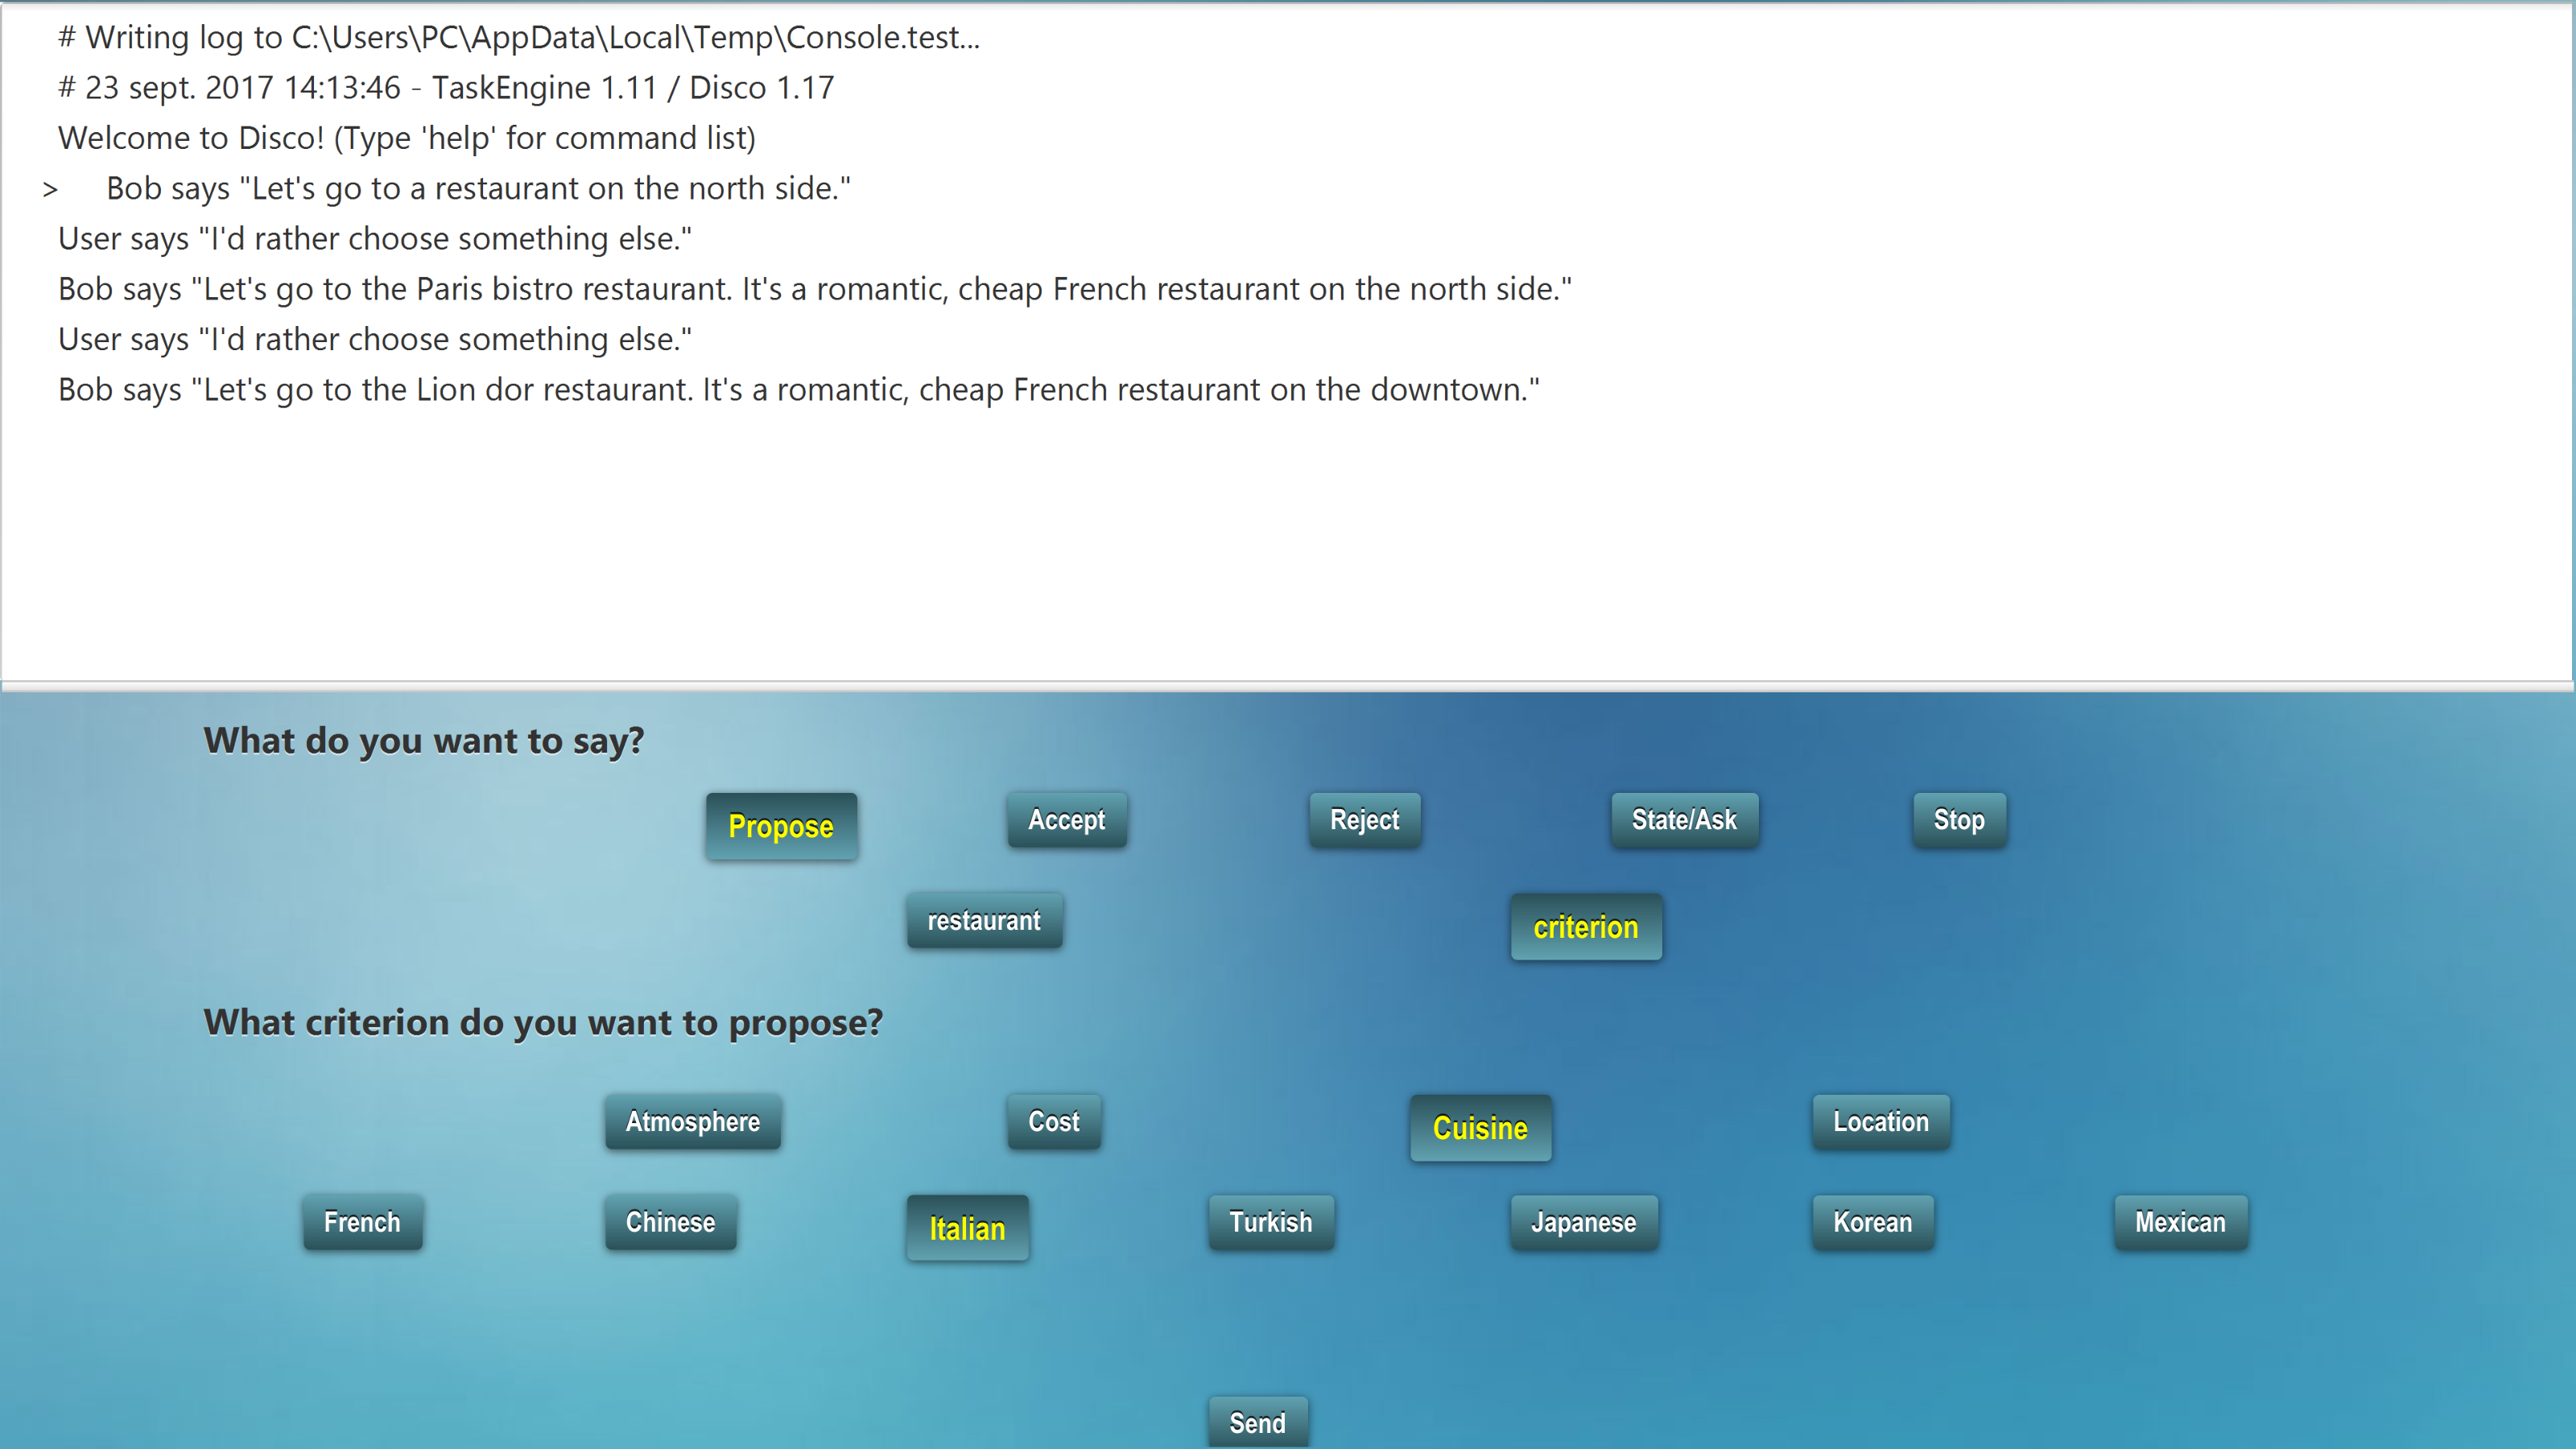
\includegraphics [width=\textwidth, height=0.4\textheight]{Figures/chap4/AH/ihm1.png}}
						\caption{GUI d'interaction avec l'agent}
						\label{fig:ihm}
					\end{figure*} 
				
				
					L'interface se présente en deux parties. La partie supérieure de l'interface affiche le cours de la négociation avec tous les messages échangés. 
					 
					Les négociateurs communiquent en utilisant les actes de dialogue que nous avons précédemment définis voir (section \ref {sec:communication}). 

					Pour ce faire, nous avons modélisé la partie inférieure de l'interface pour afficher les actes de dialogues avec toutes les combinaisons possibles. 
					Nous avons simplifié la notation des actes de dialogues pour qu'il soient compréhensibles par les participants. Par exemple, au lieu d'afficher \emph{StatePreference}, nous avons affiché un choix \emph{I (d'ont) like}.
					
					Au commencement de chaque tour, seuls les actes de dialogue sont affichés comme présenté dans la figure \ref{fig:commencement}. 
					\begin{figure*}[t]
						\centering
						\fbox{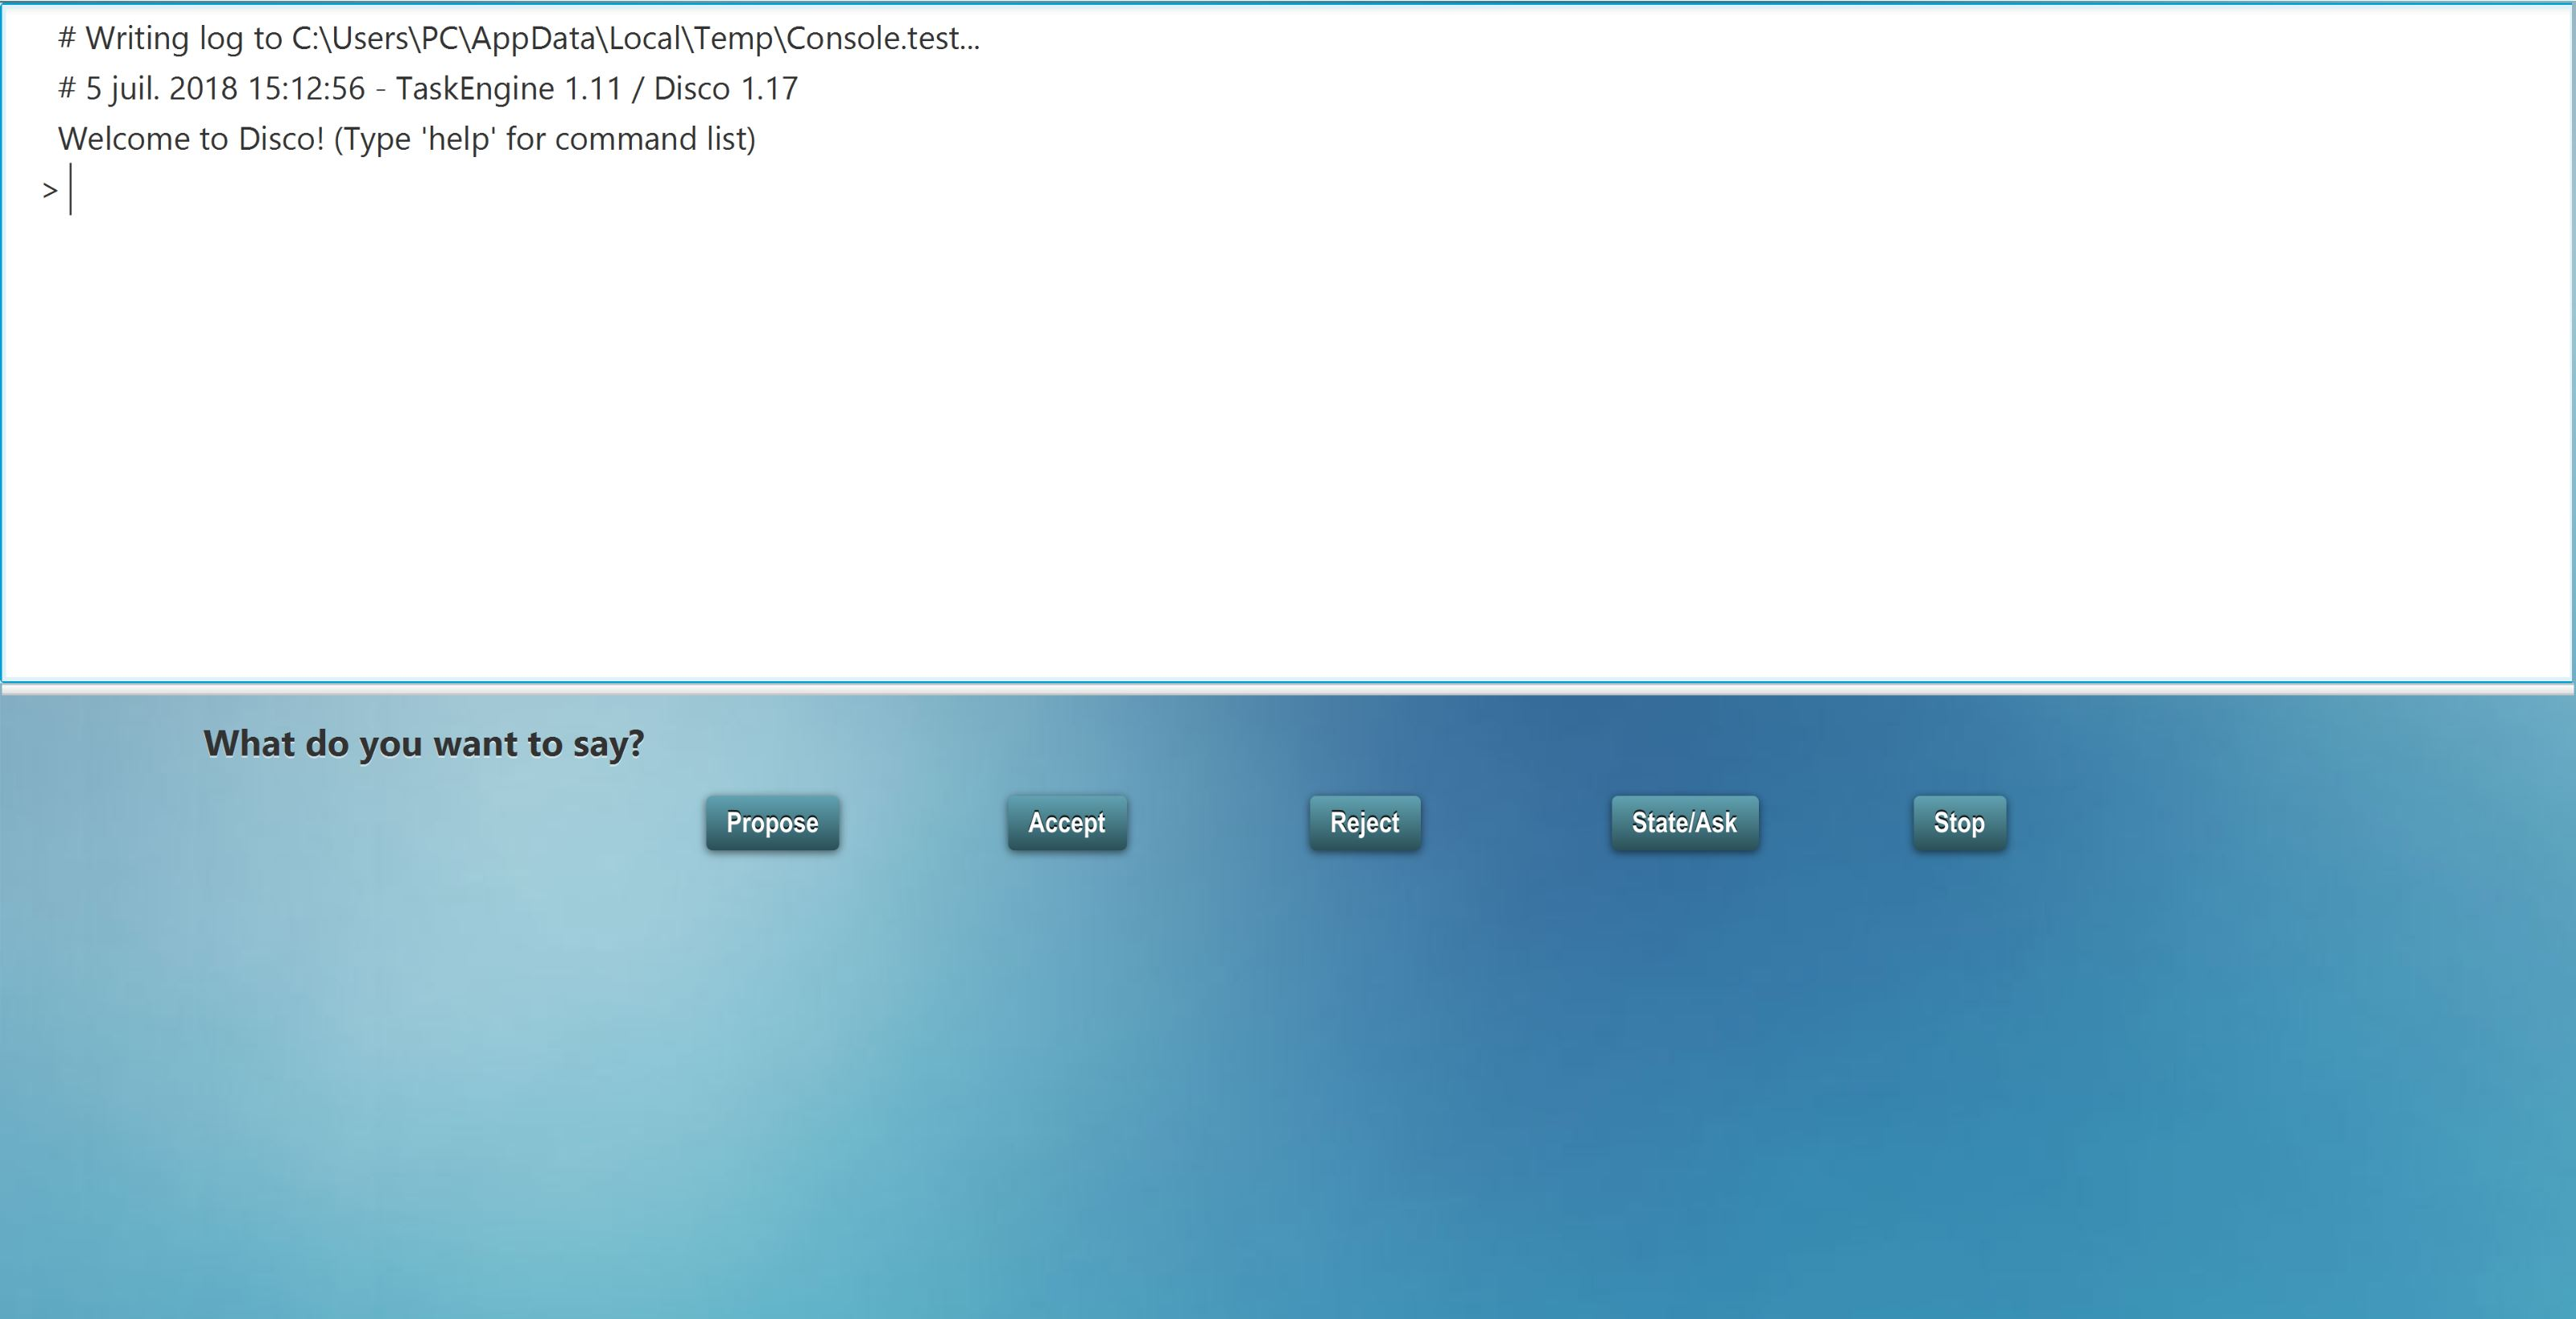
\includegraphics [width=\textwidth, height=0.25\textheight]{Figures/chap4/AH/depart.JPG}}
						\caption{GUI d'interaction avec l'agent au début de la négociation}
						\label{fig:commencement}
					\end{figure*} 
					Le participant est invité à choisir d'abord l'acte de dialogue qu'il veut annoncer. ensuite, il choisis la valeur qu'il veut exprimer avec l'acte choisi, comme présenté dans la figure \ref{fig:statIhm}.
					
					Nous avons aussi permis au participant de pouvoir utiliser les actes de dialogues combinés, par exemple \emph{Propose and counterPropose} comme présenté dans la figure 
					
					Une fois les valeurs de l'acte dialogique sont choisi, le participant envoie la requête, et notre système se charge de la formulation en langage naturel (voir section \ref{sec:formalisation} et l'affiche dans la fenêtre de dialogue. Dés la réception de la réponse du participant, l'agent affiche un message en langage naturel contenant sa réponse. 
					
					
					
					\begin{figure*}[b]
						\centering
						\fbox{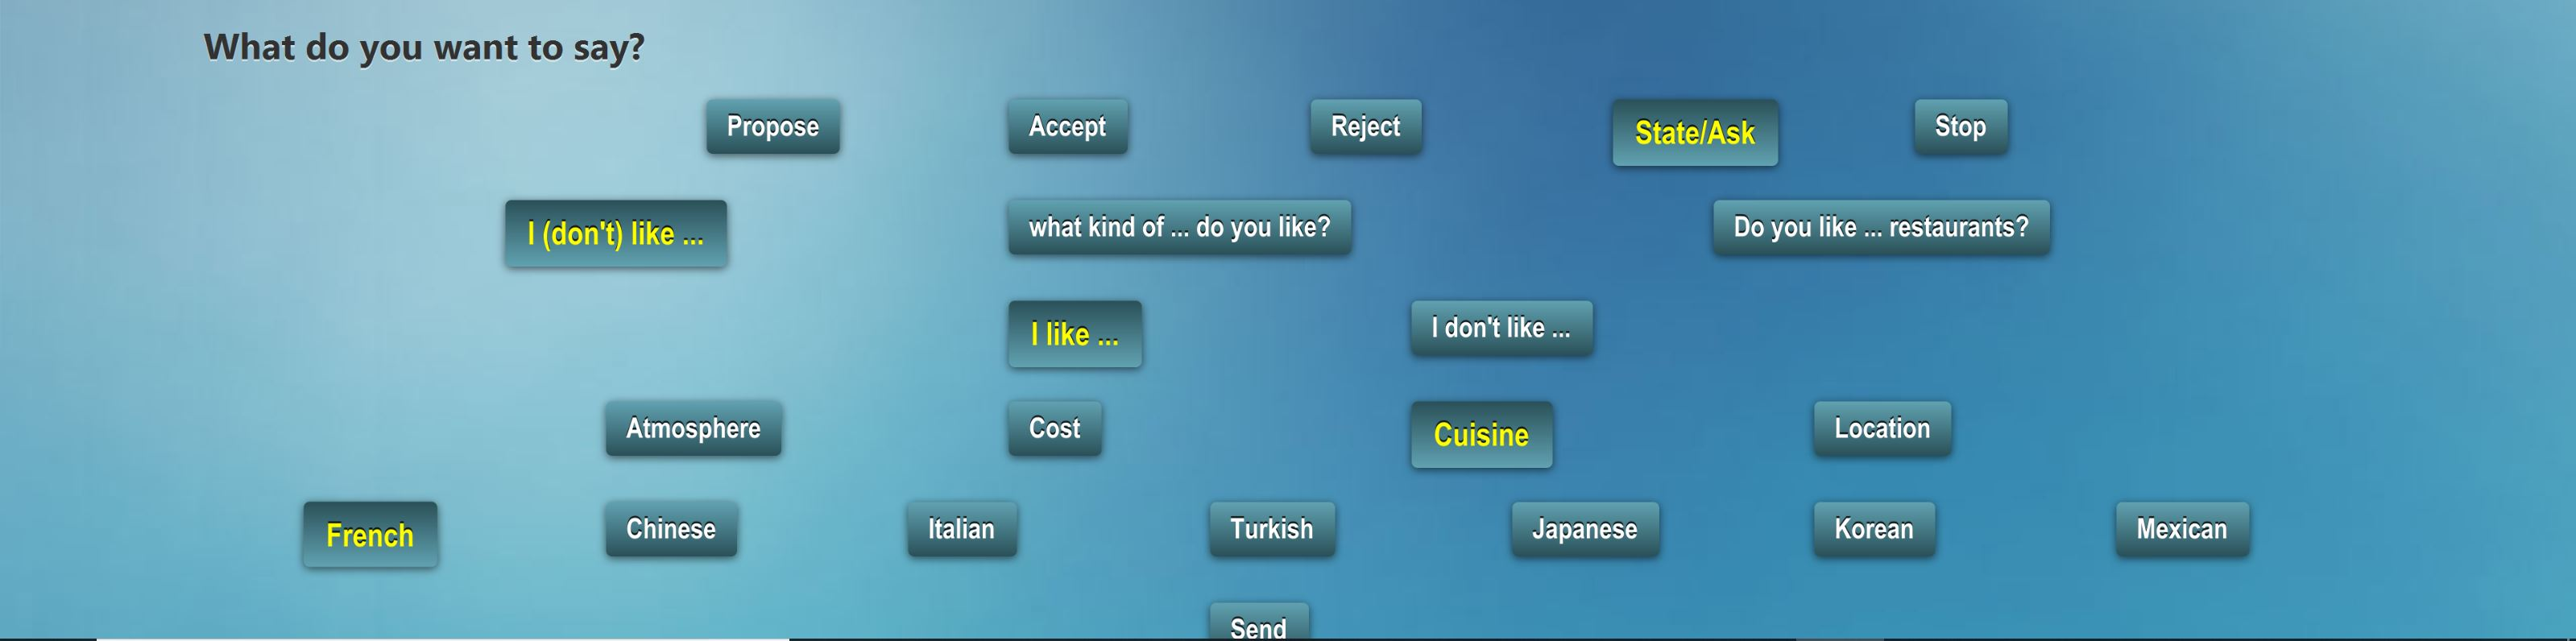
\includegraphics [width=0.85\textwidth]{Figures/chap4/AH/choixState.JPG}}
						\caption{GUI pour choisir \emph{StatePreference(French,true)} }
						\label{fig:statIhm}
					\end{figure*}
					
			\subsubsection{Procédure}
			
			Nous avons mené une étude inter-sujets où chaque participant a interagi avec les deux agents, Bob et Arthur.
			
			Au départ, le participant est invité à signer un formulaire de consentement éclairé, et  la tâche de négociation lui est expliquée. 
			Suite à cela, la  session d'entraînement commence, le participant reçoit des instructions sur l'utilisation de l'interface graphique pour interagir avec l'agent, l'expérimentateur lance la session et quitte la salle jusqu'à ce que l'entraînement soit terminé et que le participant se soit familiarisé avec l'interface. Le participant peur rappeler l'expérimentateur en cas de problèmes d'incompréhensions. 
			
			Après la formation, l'expérimentateur lance l'expérience et quitte la pièce. 
			Le participant négocie avec les deux agents. À la fin de chaque session de négociation, le participant est invité à remplir un questionnaire sur son expérience.
			
			Nous avons conçu un questionnaire permettant aux participants de rapporter leurs perceptions des comportements de l'agent lors des processus de négociation. Pour chaque hypothèse, nous avons défini deux questions avec des formulations différentes afin de ne pas biaiser les réponses des participants. En outre, nous avons défini des questions de tests pour vérifier la validité des réponses des participants. Les réponses sont données sur l'échelle de Likert.
			
			Au total, 40 participants ont participé à l'expérience. Ils ont été assignés au hasard aux conditions expérimentales.
			
			\subsubsection{Résultats}
			Nous avons effectué une étude statistique afin d'analyser la perception des comportements des agents au cours de l'interaction. Les résultats sont présentés dans la figure \ref{res}.
			
			Les participants ont majoritairement perçu que l'agent bob a tendance à mener la négociation (\emph {M = 4.40, SD = 0.9}). Ils ont également noté que Bob était exigeant (\emph {M = 3,59, SD = 1,3}) un peu égocentrique(\emph {M = 2,92, SD = 1,3}). En outre, nous avons analysé la perception des concessions faites par bob durant la négociation, les participants ont perçu que Bob faisait peu de concessions (\emph {M = 3.29, SD = 1.24}).
			
			Au contraire, les participants ont perçu le comportement d'Arthur comme suit: En moyenne, Arthur ne cherche pas à mener le dialogue (\emph {M = 1.76, SD = 1.09}). Il a un faible niveau d'exigence (\emph {M = 2.32, SD = 1.3}) et a tendance à faire des concessions (\emph {M = 3.39, SD = 1.16}). De plus, Arthur a été perçu comme prenant en compte les préférences des participants et n'est pas égoïste (\emph {M = 2.7, SD = 1.13}).
			
			La deuxième étape de notre analyse concerne l'évaluation des comportements des deux agents. Nous avons comparé le comportement de Bob et d'Arthur en utilisant un test non paramétrique de \emph{Wilcoxon pour deux échantillons appariés}. Notre première hypothèse prédit que l'agent qui exprimait des comportements de dominance Bob serait perçu comme plus égocentrique que l'agent Arthur dont les comportements sont de faible dominance. Notre analyse a confirmé notre prédiction; les participants ont perçu que Bob était plus égocentrique qu'Arthur (\emph {Z = -3,2, p = 0,001, d = -0,3}). Dans la même veine, notre seconde hypothèse a également été confirmée. Bob était perçu comme étant plus exigeant qu'Arthur avec un petit effet de taille (\emph {Z = -3.6, p <0.001, d = -0.3}).
			
			La troisième hypothèse stipulait qu'Arthur exprimerait des concessions plus importantes que Bob. L'analyse de nos données n'a pas confirmé cette hypothèse mais elle montre une tendance dans la différence de concessions (\emph {Z = -3.2, p = 0.05, d = -0.05}).
			
			La dernière hypothèse a été confirmée. Le test Wilcoxon a révélé que l'agent Bob était perçu comme significativement plus meneur dans dialogue qu'Arthur, avec une taille d'effet moyenne (\emph {Z = -3.2, p = 0.001, d = -0.6}).
			
			
			\begin{figure}[t]
				\centering
				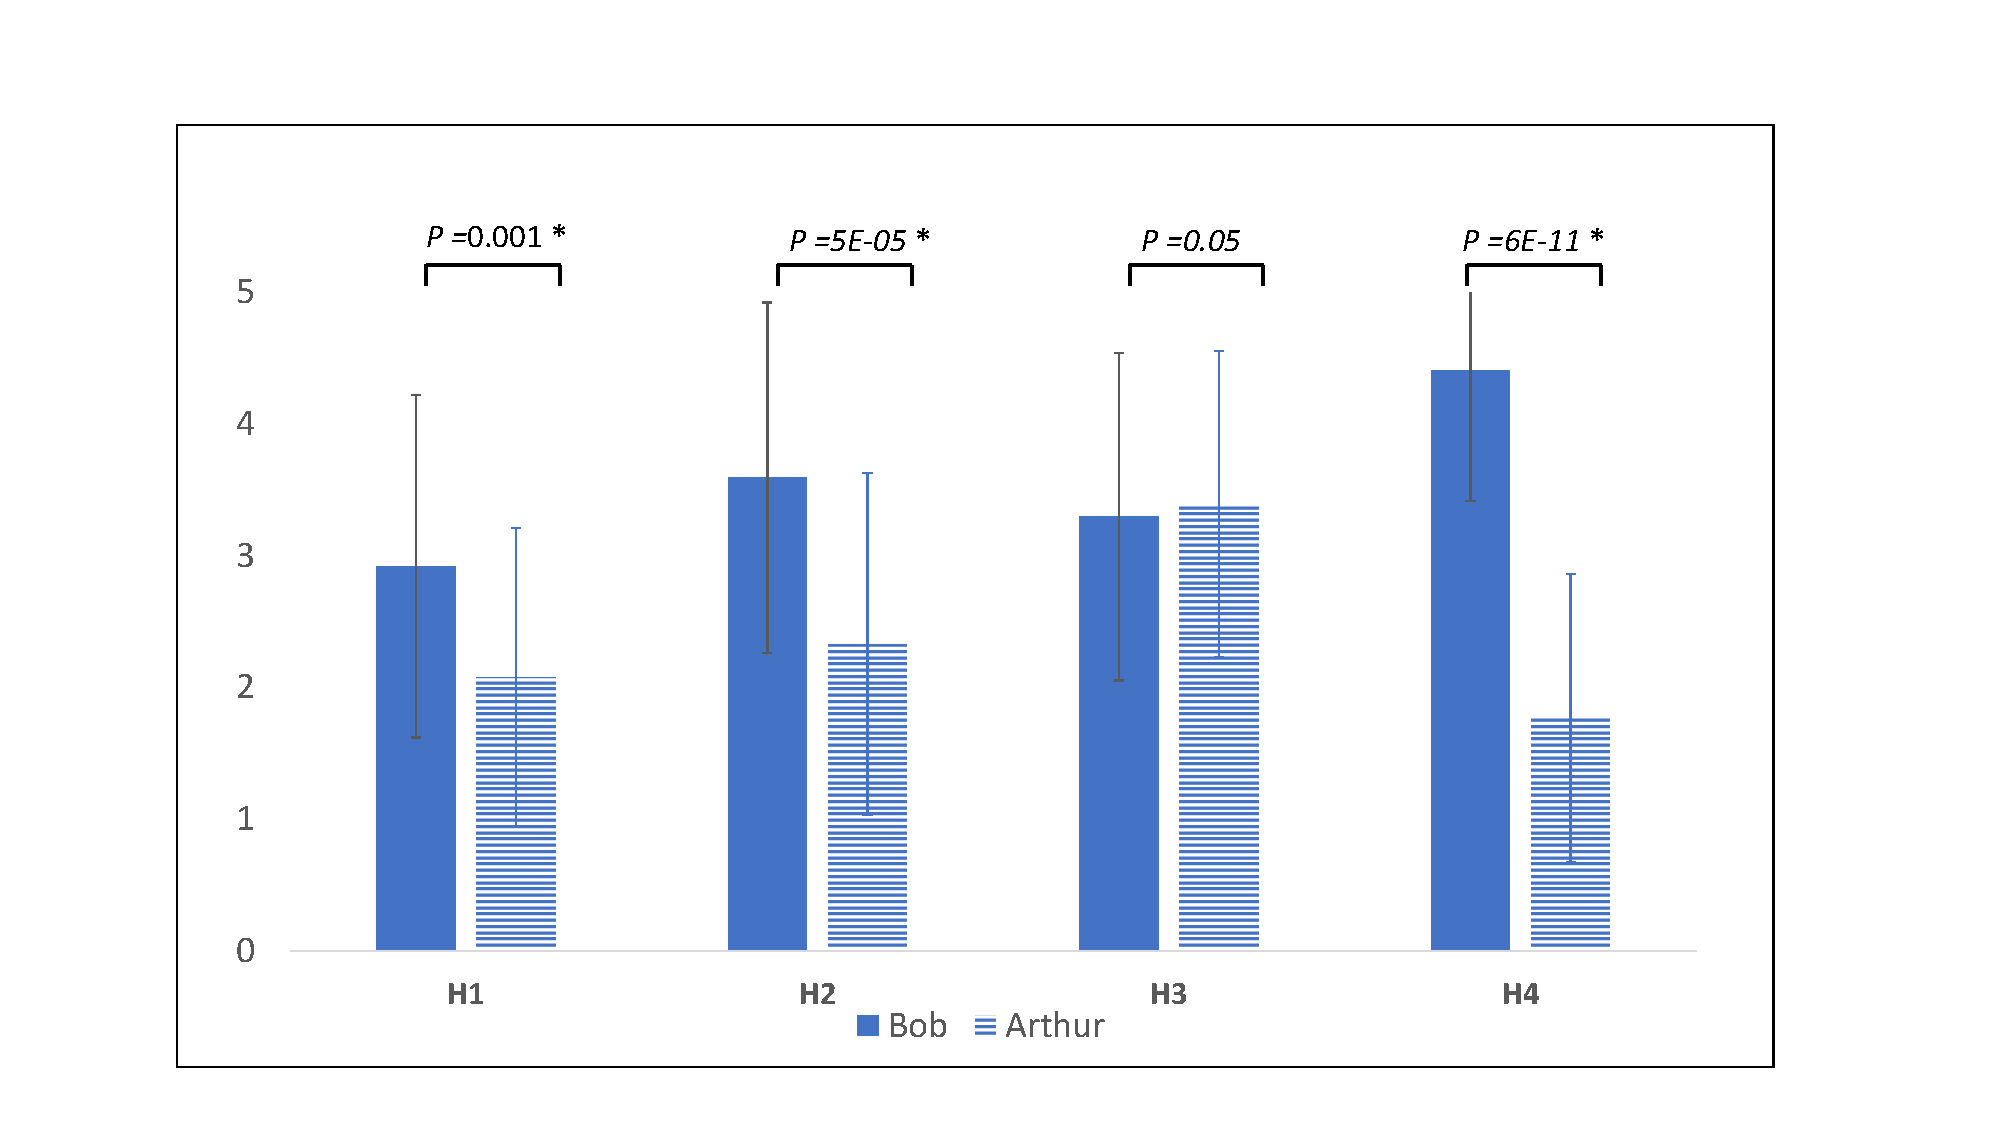
\includegraphics[width=\textwidth]{Figures/chap4/AH/res.pdf}
				\caption{Perception des comportements des agents \textit{A} et \textit{B} pour chaque hypothèse}
				\label{res}
				\end{figure}
				
				\subsubsection{Discussion}
				
				Les résultats de notre expérience appuient trois des quatre hypothèses. Les participants ont perçu Bob l'agent dominant comme meneur dans la négociation, centré sur lui-même et plus exigeant par rapport à Arthur, l'agent de faible dominance. Ces résultats sont conformes avec ceux présenté dans les travaux de Dedreu, Van Kleef et \emph{al} \cite {de1995impact, de2004influence, de2004influence} sur l'impact des comportements de dominance sur les stratégies de négociation.
				
				Cependant, la troisième hypothèse n'a pas été totalement confirmée car les participants n'ont pas perçu de différence significative dans le niveau de concession exprimé par Bob et Arthur. Ce résultat s'explique par l'impact des préférences sur le résultat de la négociation. Les préférences affectent la stratégie suivie par l'agent. Dans le cas où l'agent et l'utilisateur partagent des préférences communes, la négociation convergera rapidement et aucune confrontation des préférences ne sera expérimentée pendant la négociation. Ceci représente une limitation de notre expérience. Nous n'avons pas recueilli de connaissances préalables sur les préférences des participants. Par conséquent, nous n'avons pas été en mesure de mesurer la distance entre les préférences de l'agent et l'utilisateur et ainsi analyser l'impact des préférences sur le niveau des concessions.
				Nous n'avons pas été en mesure d'analyser les réponses à l'hypothèse 3 pour indiquer si les concessions étaient uniquement influencées par les préférences ou la relation de dominance. 
			
		\subsection{Conclusion}
			Nous avons présenté dans ce chapitre notre modèle de décision qui prend en compte la relation de dominance. En effet, l'agent construit une stratégie de négociation en fonction de sa position dans le spectre de dominance. Nous avons d'abord identifié trois principes de stratégies de négociation à partir de la littérature en psychologie sociale. Nous avons ensuite proposé un modèle computationnel de décision qui reflète chaque principe identifié.
			Ce modèle a fait l'objet de deux études pour évaluer la validité et la perception des comportements générés par le modèle décisionnel. Les résultats obtenus confirment que les participants étaient en mesure de percevoir et d'identifier les comportements de dominance exprimés par l'agent au cours de la négociation. Ces résultats bien qu'encourageants posent certaines limites. Les comportements de dominance de l'agent au cours de la négociation sont statiques et ne s'adaptent pas à ceux exprimés par son partenaire de négociation. Or, comme nous l'avons déjà présenté, la relation de dominance est dyadique, par conséquent, les comportements de dominance que l'agent expriment doivent être en fonction de ceux  exprimés par son interlocuteur.
			
			Ainsi, nos prochaines contributions auront deux objectifs. Le premier objectif est de proposer une implémentation qui va permettre à l'agent de détecter les comportements de dominance de son interlocuteur en temps réel afin de sy adapter et donc simuler une relation interpersonnelle de dominance. 
			
			La seconde contribution aura pour but d'évaluer ce modèle final dans le contexte d'une négociation entre un agent et un utilisateur humain. Nous visons à étudier si la simulation de la relation interpersonnelle de dominance aura un impact positif sur le processus de négociation en terme de gain commun et de confort ressenti à négocier avec l'agent. 
			
			
				
				